\documentclass[a4paper,12pt]{article} % Utilisation de la classe article
\usepackage[utf8]{inputenc}  % LaTeX, comprends les accents !
\usepackage[T1]{fontenc}  % Police contenant les caractères français
\usepackage[french]{babel}  % Le document est en français
\usepackage{fullpage}  % pour les marges
\usepackage{graphicx}  % pour inclure des images
\usepackage{lmodern}  % font type
\usepackage{datetime}  % pour la date
\usepackage[shortlabels]{enumitem}  % pour les listes numérotées
\setlist[itemize,1]{label={\color{gray}\small \textbullet}} % customises itemize default -
\usepackage{xcolor} % colour customisation, extends to tables with {colortbl}
\usepackage{url}  % pour les url
\usepackage[breaklinks]{hyperref} % pour casser les liens hypertextes
\usepackage{breakurl} % pour casser les liens hypertextes
\usepackage{amsmath} % pour les formules mathématiques
\usepackage{amssymb}
\usepackage{mathtools}
\usepackage{amsthm}
\usepackage[]{mdframed} % Framing for environments
\usepackage{mathrsfs}
\usepackage{tcolorbox} % Pour encadrer
\tcbuselibrary{skins, breakable} % Pour des boîtes personnalisables
\usepackage{cancel}
\usepackage{array} % à mettre dans le préambule
\renewcommand{\arraystretch}{1.5} % augmente la hauteur des lignes de 50%
\usepackage{placeins} % à mettre dans le préambule
\DeclareMathOperator*{\argmax}{arg\,max}
\DeclareMathOperator*{\argmin}{arg\,min}
\usepackage{bigints}
\usepackage{tikz-3dplot}
\usetikzlibrary{3d, calc, angles, quotes} % fichier contenant les packages et les commandes personnalisées
\makeatletter
% Custom Commands for fast mathematical notation --------------------------------
% General shortcuts
\newcommand{\scr}[1]{\mathscr{#1}} % Script font shortcut
\newcommand{\scrF}{\mathscr{F}} % Script font shortcut
\newcommand{\bb}[1]{\mathbb{#1}} % Blackboard bold shortcut
\newcommand{\ol}[1]{\overline{#1}} % Overline shortcut
\newcommand{\ul}[1]{\underline{#1}} % Underline shortcut
\newcommand{\act}{\circlearrowleft} % Action symbol
\newcommand{\vphi}{\varphi} 
\newcommand{\cxi}{\langle\xi\rangle} % <xi> poids pour les Sobolevs
\newcommand{\Dx}{\Delta x}
\newcommand{\Dy}{\Delta y}
\newcommand{\Uij}{U_{ij}}
\newcommand{\omb}{\overline{\Omega}} % Adhérence d'Omega
\newcommand{\eqxi}{(1+\n{\xi}^2)} % écrit (1 + ∣ξ∣^2) pour les Sobolevs
\newcommand{\RRd}{(\R \times \R^d)}
\newcommand{\et}{e^{t\triangle}}
\newcommand{\ijn}{(i,j)\in}

% Interval notation
\newcommand{\oo}[1]{\mathopen{}\left]#1\right[\mathclose{}} % Open interval % chktex 9
\newcommand{\ooo}{\mathopen{}\left]0,T\right[\mathclose{}} % Open interval % chktex 9
\newcommand{\of}[1]{\mathopen{}\left]#1\right]\mathclose{}} % Half-open interval (open first) % chktex 9 % chktex 10
\newcommand{\fo}[1]{\mathopen{}\left[#1\right[\mathclose{}} % Half-open interval (open last)
\newcommand{\ff}[1]{\mathopen{}\left[#1\right]\mathclose{}} % Closed interval % chktex 9
\newcommand{\ffo}{\mathopen{}\left[0,T\right]\mathclose{}} % Closed interval % chktex 9

% Set notation
\newcommand{\R}{\mathbb{R}} % Real numbers
\newcommand{\Z}{\mathbb{Z}} % Integers
\newcommand{\N}{\mathbb{N}} % Natural numbers
\newcommand{\C}{\mathscr{C}} % Fonctions continues
\newcommand{\Q}{\mathbb{Q}} % Rational numbers
\newcommand{\D}{\mathscr{D}} % Ensemble des fonctions tests
\newcommand{\Dp}{\mathscr{D^{'}}} % Ensemble des distributions 
\newcommand{\Sp}{\mathscr{S}^{'}} % Distributions tempérées
\newcommand{\scrS}{\mathscr{S}} % Classe de Schwartz
\newcommand{\Hs}{H^s(\R^d)}
\newcommand{\bbR}{\mathbb{R}} % Real numbers
\newcommand{\bbZ}{\mathbb{Z}} % Integers
\newcommand{\bbN}{\mathbb{N}} % Natural numbers
\newcommand{\bbC}{\mathbb{C}} % Complex numbers
\newcommand{\bbQ}{\mathbb{Q}} % Complex numbers
\newcommand{\scrP}{\mathscr{P}} % Set of subsets
\newcommand{\barR}{\overline{\bb{R}}} % R with infinities
\newcommand{\gln}{\text{GL}_n} % General linear group of degree n
\newcommand{\glx}[1]{\text{GL}_{#1}} % General linear group
%
\newcommand{\sub}{\subset} % Subset
\newcommand{\cequiv}[1]{\mathopen{}[#1\mathclose{}]} % Equivalence class
\newcommand{\restr}[2]{#1\mathop{}\!|_{#2}} % Restriction
\newcommand{\adh}[1]{\mathring{#1}} % Adherence
\newcommand{\Adh}[1]{\mathring{\overbrace{#1}}} % Big adherence
\newcommand{\comp}[1]{{#1}^C} % Complementary of a set

% Differential notation
\newcommand{\der}{\mathop{}\!{d}} % Differential operator
\newcommand{\p}{\mathop{}\!{\partial}} % Partial derivative operator
\providecommand{\dpar}[2]{\frac{\partial{#1}}{\partial{#2}}}

% Topology notation
\newcommand{\bolo}[1]{B\left({#1}\mathopen{}\right[\mathclose{}} % Open ball
\newcommand{\bolf}[1]{B\left({#1}\mathopen{}\right]\mathclose{}} % Closed ball

% Limits notation
\newcommand{\limi}{\underline{\lim}}
\newcommand{\lims}{\overline{\lim}}

% Norm notation
\newcommand{\norm}{\mathcal{N}} % Norm
\newcommand{\nn}[1]{\mathopen{}\left\|#1\right\|\mathclose{}} % Double bar norm
\newcommand{\nnn}[1]{\mathopen{}\left\||#1|\right\|\mathclose{}} % Double bar norm
\newcommand{\n}[1]{\mathopen{}\left|#1\right|\mathclose{}} % Single bar norm


% Other operators
\providecommand{\1}{\mathds{1}} % Identity operator
\DeclareMathOperator{\im}{\mathsf{Im}} % Imaginary part
\DeclareRobustCommand{\re}{\mathsf{Re}} % Real part
\DeclareMathOperator{\vect}{\mathsf{Vect}} % Vector space
\DeclareMathOperator{\diam}{\mathsf{Diam}} % Diameter
\DeclareMathOperator{\orb}{\mathsf{orb}} % Orbit
\DeclareMathOperator{\st}{\mathsf{st}} % Standard part
\DeclareMathOperator{\spr}{\mathsf{SP_{\bb{R}}}} % Real spectrum
\DeclareMathOperator{\aut}{\mathsf{Aut}} % Automorphism group
\DeclareMathOperator{\bij}{\mathsf{Bij}} % Bijection group
\DeclareMathOperator{\rank}{\mathsf{rank}} % Rank
\DeclareMathOperator{\tr}{\mathsf{tr}} % Trace
\DeclareMathOperator{\id}{\mathsf{Id}} % Identity
\DeclareMathOperator{\var}{\mathsf{Var}} % Variance
\DeclareMathOperator{\cov}{\mathsf{Cov}} % Covariance
\DeclareFontFamily{U}{mathx}{}
\DeclareFontShape{U}{mathx}{m}{n}{<-> mathx10}{}
\DeclareSymbolFont{mathx}{U}{mathx}{m}{n}
\DeclareMathAccent{\widecheck}{0}{mathx}{"71}
\providecommand{\B}{\mathsf{B}} % Bold symbol

\usepackage{dsfont}
\newcommand{\one}{\mathds{1}}

\newcommand{\smol}[1]{\text{\scriptsize{#1}}}

\newcommand{\bleu}[1]{{\color{blue} #1}}
\newcommand{\ver}[1]{{\color{green} #1}}
\newcommand{\rouge}[1]{{\color{red}#1}}
\newcommand{\orange}[1]{{\color{orange}#1}}



\makeatother % Plein de macro pour les symboles, hésite pas à en rajouter/modifier si tu les aimes pas xD (c'est les miennes, je ne veux pas te les imposer)

\newtheoremstyle{default}{\topsep}{\topsep}%
{}% Body font
{}% Indent amount (empty = no indent, \parindent = para indent)
{\sffamily\bfseries}% Thm head font
{.}% Punctuation after thm head
{ }% Space after thm head (\newline = linebreak)
{\thmname{#1}\thmnumber{~#2}\thmnote{~#3}}% Thm head spec

\newtheoremstyle{nonum}{\topsep}{\topsep}%
{}%
{}%
{\sffamily\bfseries}%
{.}%
{ }%
{\thmname{#1}}%

\newcommand{\mytheorem}[5]{%
	\ifstrequal{#5}{o}{%
		\newmdtheoremenv[
		hidealllines=true,
		skipabove=0pt,
		innertopmargin=-5pt,
		innerbottommargin=2pt,
		linewidth=1pt,
        innerleftmargin=0pt,
		]{#1}[#4]{#2}%
	}{% Dependant counter
		\newmdtheoremenv[
		hidealllines=true,
		skipabove=0pt,
		innertopmargin=-5pt,
		innerbottommargin=2pt,
		linewidth=1pt,
		linecolor=#3,
        innerleftmargin=0pt,
		]{#1}{#2}[#4]%
	}%
}

% Custom Global Theorems --------------------------------------------------------
\theoremstyle{default}
\newtoggle{showsolutions}
\newcounter{oc-counter}
\mytheorem{oc-proposition}{Proposition}{divergent-denim}{oc-counter}{o}
\mytheorem{oc-propdef}{Proposition - Définition}{divergent-denim}{oc-counter}{o}
\mytheorem{oc-theorem}{Théorème}{divergent-denim}{oc-counter}{o}
\mytheorem{oc-lemme}{Lemme}{quadratic-quartz}{oc-counter}{o}
\mytheorem{oc-example}{Exemple}{quadratic-quartz}{oc-counter}{o}
\mytheorem{oc-remark}{Remarque}{matrix-mist}{oc-counter}{o}
\mytheorem{oc-exercise}{Exercice}{calculus-coral}{oc-counter}{o}
\mytheorem{oc-definition}{Definition}{algebraic-amber}{oc-counter}{o}
\mytheorem{oc-corollaire}{Corollaire}{violet}{oc-counter}{o}
\counterwithin{oc-counter}{subsection}



\makeatletter


%--------------------------------------------------------------------------------
\newcommand{\cv}{\longrightarrow}
\newcommand{\cvn}{\underset{n\to\infty}{\cv}}
\newcommand{\cvps}{{\overset{\text{p.s.}}{\longrightarrow}}}
\newcommand{\cvpsn}{\underset{n\to\infty}{\cvps}}
\newcommand{\cvp}{{\overset{\mathbb{P}}{\longrightarrow}}}
\newcommand{\cvpn}{\underset{n\to\infty}{\cvp}}
\newcommand{\cvlp}{{\overset{\mathcal{L}^{p}}{\longrightarrow}}}
\newcommand{\cvlpn}{\underset{n\to\infty}{\cvlp}}
\newcommand{\cvd}{{\overset{(\mathcal{D})}{\longrightarrow}}}
\newcommand{\cvdn}{\underset{n\to\infty}{\cvd}}
\newcommand{\cvlaw}{{\overset{(\mathscr{L})}{\longrightarrow}}}
\newcommand{\cvlawn}{\underset{n\to\infty}{\cvlaw}}
\newcommand{\iid}{\text{i.i.d.}}




%--------------------------------------------------------------------------------
% Custom Per Subject Theorems
%--------------------------------------------------------------------------------

% -- Numerotation classique des theoremes
\theoremstyle{default}
\mytheorem{definition}{Définition}{algebraic-amber}{}{o}
\mytheorem{exs}{Exemples}{matrix-mist}{}{o}
\mytheorem{corollaire}{Corollaire}{violet}{}{o}
\mytheorem{lemme}{Lemme}{}{}{o}
\mytheorem{proposition}{Proposition}{verdant}{}{o}
\mytheorem{theorem}{Théorème}{astral}{}{o}

% -- Theoremes sans numeros -- %
\theoremstyle{nonum}
\mytheorem{nodefinition}{Définition}{algebraic-amber}{}{o}
\mytheorem{noproposition}{Proposition}{verdant}{}{o}
\mytheorem{noexample}{Exemple}{matrix-mist}{}{o}
\mytheorem{notheorem}{Théorème}{astral}{}{o}
\mytheorem{norappel}{Rappel}{red}{}{o}
\mytheorem{noremark}{Remarque}{}{}{o}
\mytheorem{nopropriete}{Propriété}{}{}{o}
\mytheorem{nonotation}{Notation}{}{}{o}
\makeatother


\begin{document}
\begin{titlepage}
\begin{center}
\vspace{2cm}
%\textsc{ Oregon State University}\\[1.5cm]

\includegraphics[width=0.4\textwidth]{./Images/UM1.png}~\\[1cm]
\vspace{2cm}

% Title
\hrule
\vspace{.5cm}
{\huge\bfseries{Problèmes Shape-from-Shading\\Projet de M1}} % title of the report
\vspace{.5cm}

\hrule
\vspace{1.5cm}

\textsc{\textbf{Auteurs}}\\
\vspace{.5cm}
\centering

% add your name here
BIGEY Raphaël \\
TARI Julien


\vspace{1cm}

\textsc{\textbf{Encadrante}}\\
\vspace{.5cm}
\centering

% add your name here
GUERAND Jessica
\vspace{4cm}

\centering \today % Dags dato
\end{center}
\end{titlepage}  % page de garde

\tableofcontents  % Table des matières
\newpage

\section{Introduction}
\subsection{Présentation du Shape-from-Shading}

Le Shape-from-Shading (SFS) est un problème fondamental en vision par ordinateur. Il consiste à reconstruire en 3D la surface d’un objet à partir des variations d’intensité lumineuse observées dans une image. Sous certaines hypothèses, ces variations permettent d’estimer les pentes de la surface, et donc de reconstruire la géométrie de l'objet. Lorsqu'on le formule d'un point de vue mathématique, on est amené à étudier une équation aux dérivées partielles (EDP) non linéaire d'ordre 1. Sa solution donne alors la hauteur ou la profondeur de l'objet étudié. 
Nous donnons ici un exemple de SFS appliqué à la reconstruction d'un vase artificiel. Cet exemple est issu de \cite{ref_vase}.

% insert 2 side by side redimensionned images
\begin{figure}[!htb]
    \begin{minipage}[t]{0.5\textwidth}
        \centering
        \fbox{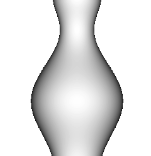
\includegraphics[width=.46\linewidth,height=4cm]{./Images/vase_tuto.png}}
        \caption{Intensité lumineuse d'un vase}\label{Fig:int_vase2}
    \end{minipage}\hfill
    \begin{minipage}[t]{0.5\textwidth}
        \centering
        \fbox{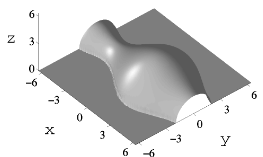
\includegraphics[width=.7\linewidth,height=4cm]{./Images/vase_tutor.png}}
        \caption{Vase reconstruit}\label{Fig:vase_tutor}
    \end{minipage}
\end{figure}

\subsection{Contexte historique}
Le problème du Shape-from-Shading est apparu dans les années 1970, à une époque où les chercheurs en vision par ordinateur commençaient à s’intéresser à la manière dont la lumière et l’ombre pouvaient être exploitées pour comprendre la géométrie des scènes. À cette époque, le SFS consistait principalement à reconstituer la forme d’objets à partir d’images en niveaux de gris. Cependant, avec le développement des technologies, plusieurs variantes du Shape-from-Shading ont été développées pour faire face à des situations plus complexes rencontrées dans des scènes réelles. On distingue par exemple 
\begin{itemize}
    \item Le \textbf{SFS classique}, avec une seule source lumineuse et un unique objet dans la scène. 
    \item Le \textbf{SFS à plusieurs lumières}, où l'objet est éclairé par plusieurs lumières. La multiplicité des sources de lumière permet d'obtenir plus d'informations sur l'objet. Cependant, la modélisation devient bien plus compliquée.
    \item Le \textbf{SFS à plusieurs objets}, qui s’intéresse à la reconstruction de scènes qui contiennent plusieurs objets qui peuvent en partie se chevaucher/superposer/cacher du point de vue de l'observateur.
    \item Le \textbf{SFS non lambertien}, qui tient compte des matériaux de l'objet. 
\end{itemize}

Ces différentes variantes démontrent la diversité des problèmes de SFS. De nos jours, l'utilisation du Shape-from-Shading est assez spécifique mais plutôt utile dans l'imagerie médicale et notamment dans la radiographie. Celui-ci intervient aussi dans l'inspection industrielle. En effet, le SFS est utilisé dans le contrôle qualité de pièces mécaniques (trouver des aspérités/irrégularités à la surface d'un objet). 
L’un des travaux fondateurs dans ce domaine est celui de B.K.P. Horn en 1975 \cite{Horn 1975}, qui a posé les bases mathématiques du problème en liant l’intensité lumineuse d’un pixel à l’orientation locale de la surface. Il voulait notamment appliquer le SFS à la représentation de la lune et à la vision par robot. Par \og vision par robot \fg{} nous entendons la capacité des machines à détecter et analyser des images ou des vidéos afin de prendre des décisions.


\subsection{Mise en équation du problème} 

Comme nous l'avons énoncé plus haut, le problème de SFS se réduit, sous les bonnes hypothèses, à résoudre une EDP non linéaire d'ordre 1. Nous souhaitons dans cette partie présenter les hypothèses de base afin de comprendre pourquoi une telle équation modélise correctement le problème. Cette modélisation est issue des travaux de Horn dans \cite{Horn 1986}.\\

Une \textbf{surface lambertienne} est une surface suivant la loi de Lambert. C'est-à-dire qu'elle ne produit pas de lumière spéculaire mais aussi que la quantité de lumière renvoyée est proportionnelle au cosinus de l’angle entre la lumière incidente et la normale à la surface. 

Un \textbf{angle solide} est une mesure de l'étendue d'un objet vu depuis un point donné. On le note $S$ et on l'exprime en stéradians (noté \(sr\)). Il est défini comme le rapport entre l'aire d'une portion de surface sphérique interceptée par un cône (ou toute forme tridimensionnelle) et le carré du rayon de la sphère: 
\begin{equation*}
    S=\frac{A \cos\left(\theta\right)}{r^2},
\end{equation*}
où $A$ représente l'aire de l'objet et $r$ la distance objet-observateur.

Par exemple, si on prend un disque de rayon 1m, situé à 1m de l'observateur, on aura $S={\pi} \ sr$. Si ce même disque se situe à 2m, on aura $S=\frac{\pi}{4}$ \(sr\). Il sera donc visuellement 4 fois plus petit. Enfin, si on incline le disque dans l'espace, visuellement on verra une ellipse et aura un angle solide plus faible.

\hspace{1.5cm}
\tdplotsetmaincoords{70}{110} % Adjust camera angles (theta, phi)
\begin{tikzpicture}[tdplot_main_coords, scale=3]
    % Base circle (cutting plane)
    \draw[thick] (0,0,0) circle (1);

    % Hemisphere (3D surface)
    \foreach \phi in {0,10,...,360} { % Longitude lines
        \draw[gray!50] 
            plot[domain=0:90, smooth, variable=\theta] 
            ({cos(\phi)*sin(\theta)}, {sin(\phi)*sin(\theta)}, {cos(\theta)});
    }
    \foreach \theta in {15,35,55,75} { % Latitude lines
        \draw[gray!50] 
            plot[domain=-180:180, smooth, variable=\phi] 
            ({cos(\phi)*sin(\theta)}, {sin(\phi)*sin(\theta)}, {cos(\theta)});
    }

    % --- Corrected curved rectangle patch ---
    \def\phiStart{-37}  % Longitude range
    \def\phiEnd{-22}
    \def\thetaStart{41} % Latitude range (from pole)
    \def\thetaEnd{53}

    % Calculate the four corners of the curved rectangle
    \coordinate (A) at ({cos(\phiStart)*sin(\thetaStart)}, {sin(\phiStart)*sin(\thetaStart)}, {cos(\thetaStart)});
    \coordinate (B) at ({cos(\phiEnd)*sin(\thetaStart)}, {sin(\phiEnd)*sin(\thetaStart)}, {cos(\thetaStart)});
    \coordinate (C) at ({cos(\phiEnd)*sin(\thetaEnd)}, {sin(\phiEnd)*sin(\thetaEnd)}, {cos(\thetaEnd)});
    \coordinate (D) at ({cos(\phiStart)*sin(\thetaEnd)}, {sin(\phiStart)*sin(\thetaEnd)}, {cos(\thetaEnd)});
    
    % Draw the curved patch
    \filldraw[red!20, draw=red, thick]
        plot[domain=\thetaStart:\thetaEnd, smooth, variable=\theta]
        ({cos(\phiStart)*sin(\theta)}, {sin(\phiStart)*sin(\theta)}, {cos(\theta)}) --
        plot[domain=\phiStart:\phiEnd, smooth, variable=\phi]
        ({cos(\phi)*sin(\thetaEnd)}, {sin(\phi)*sin(\thetaEnd)}, {cos(\thetaEnd)}) --
        plot[domain=\thetaEnd:\thetaStart, smooth, variable=\theta]
        ({cos(\phiEnd)*sin(\theta)}, {sin(\phiEnd)*sin(\theta)}, {cos(\theta)}) --
        plot[domain=\phiEnd:\phiStart, smooth, variable=\phi]
        ({cos(\phi)*sin(\thetaStart)}, {sin(\phi)*sin(\thetaStart)}, {cos(\thetaStart)}) --
        cycle;
    

    % Add red "S" label
    \node[red] at ({cos((\phiStart+\phiEnd)/2)*sin((\thetaStart+\thetaEnd)/2)}, 
    {sin((\phiStart+\phiEnd)/2)*sin((\thetaStart+\thetaEnd)/2)}, 
    {cos((\thetaStart+\thetaEnd)/2)}) {\large \(S\)};
    
    % --- Calculate projected rectangle corners ---
    \def\projectionDistance{1.5} % Distance for the projected rectangle
    
    % Project corner A
    \pgfmathsetmacro{\Ax}{cos(\phiStart)*sin(\thetaStart)}
    \pgfmathsetmacro{\Ay}{sin(\phiStart)*sin(\thetaStart)}
    \pgfmathsetmacro{\Az}{cos(\thetaStart)}
    \pgfmathsetmacro{\scale}{\projectionDistance/\Az}
    \coordinate (A') at ({\scale*\Ax}, {\scale*\Ay}, {\projectionDistance});
    
    % Project corner B
    \pgfmathsetmacro{\Bx}{cos(\phiEnd)*sin(\thetaStart)}
    \pgfmathsetmacro{\By}{sin(\phiEnd)*sin(\thetaStart)}
    \pgfmathsetmacro{\Bz}{cos(\thetaStart)}
    \pgfmathsetmacro{\scale}{\projectionDistance/\Bz}
    \coordinate (B') at ({\scale*\Bx}, {\scale*\By}, {\projectionDistance});
    
    % Project corner C
    \pgfmathsetmacro{\Cx}{cos(\phiEnd)*sin(\thetaEnd)}
    \pgfmathsetmacro{\Cy}{sin(\phiEnd)*sin(\thetaEnd)}
    \pgfmathsetmacro{\Cz}{cos(\thetaEnd)}
    \pgfmathsetmacro{\scale}{\projectionDistance/\Cz}
    \coordinate (C') at ({\scale*\Cx}, {\scale*\Cy}, {\projectionDistance});
    
    % Project corner D
    \pgfmathsetmacro{\Dx}{cos(\phiStart)*sin(\thetaEnd)}
    \pgfmathsetmacro{\Dy}{sin(\phiStart)*sin(\thetaEnd)}
    \pgfmathsetmacro{\Dz}{cos(\thetaEnd)}
    \pgfmathsetmacro{\scale}{\projectionDistance/\Dz}
    \coordinate (D') at ({\scale*\Dx}, {\scale*\Dy}, {\projectionDistance});
    
    % Draw the projected rectangle
    \filldraw[blue!20, draw=blue, thick] (A') -- (B') -- (C') -- (D') -- cycle;
    
    % Draw projection lines (dotted lines from origin through curved rectangle corners to projected rectangle corners)
    \draw[dashed, thick] (0,0,0) -- (A) -- (A');
    \draw[dashed, thick] (0,0,0) -- (B) -- (B');
    \draw[dashed, thick] (0,0,0) -- (C) -- (C');
    \draw[dashed, thick] (0,0,0) -- (D) -- (D');

    \pgfmathsetmacro{\midPhi}{(\phiStart+\phiEnd)/2}
    \pgfmathsetmacro{\midTheta}{(\thetaStart+\thetaEnd)/2}
    % Calculate projected center (P') and patch center (P)
    \coordinate (P) at ({cos(\midPhi)*sin(\midTheta)}, {sin(\midPhi)*sin(\midTheta)}, {cos(\midTheta)});
    \pgfmathsetmacro{\scale}{\projectionDistance/cos(\midTheta)}
    \coordinate (P') at ({\scale*cos(\midPhi)*sin(\midTheta)}, {\scale*sin(\midPhi)*sin(\midTheta)}, {\projectionDistance});
    
    % Draw blue projection line (r)
    \draw[<->, thick, blue] (0,0,0) -- (P') node[very near end, below] {\(r\)};
    
    % --- Calculate surface normal and incidence angle ---
    % For a flat rectangle in 3D, we need two edge vectors to calculate the normal
    % Edge vector 1: from A' to B'
    \pgfmathsetmacro{\edgeOneX}{\scale*\Bx - \scale*\Ax}
    \pgfmathsetmacro{\edgeOneY}{\scale*\By - \scale*\Ay}
    \pgfmathsetmacro{\edgeOneZ}{0} % Both points have same z-coordinate
    
    % Edge vector 2: from A' to D'
    \pgfmathsetmacro{\edgeTwoX}{\projectionDistance/\Dz*\Dx - \scale*\Ax}
    \pgfmathsetmacro{\edgeTwoY}{\projectionDistance/\Dz*\Dy - \scale*\Ay}
    \pgfmathsetmacro{\edgeTwoZ}{0} % Both points have same z-coordinate
    
    % Cross product to get normal vector (simplified since z-components are 0)
    \pgfmathsetmacro{\normalX}{0}
    \pgfmathsetmacro{\normalY}{0}
    \pgfmathsetmacro{\normalZ}{1} % The rectangle is in a plane parallel to xy-plane, so normal is (0,0,1)
    
    % Actually, let's use the correct normal for the projected rectangle
    % Since all points have the same z-coordinate, the normal is simply (0,0,1)
    
    % Center of the projected rectangle
    \pgfmathsetmacro{\centerX}{(\scale*\Ax + \scale*\Bx + \projectionDistance/\Cz*\Cx + \projectionDistance/\Dz*\Dx)/4}
    \pgfmathsetmacro{\centerY}{(\scale*\Ay + \scale*\By + \projectionDistance/\Cz*\Cy + \projectionDistance/\Dz*\Dy)/4}
    \pgfmathsetmacro{\centerZ}{\projectionDistance}
    
    % Vector from origin to rectangle center (incident ray direction)
    \pgfmathsetmacro{\incidentX}{\centerX}
    \pgfmathsetmacro{\incidentY}{\centerY}
    \pgfmathsetmacro{\incidentZ}{\centerZ}
    
    % Normalize the incident vector
    \pgfmathsetmacro{\incidentLength}{sqrt(\incidentX*\incidentX + \incidentY*\incidentY + \incidentZ*\incidentZ)}
    \pgfmathsetmacro{\incidentUnitX}{\incidentX/\incidentLength}
    \pgfmathsetmacro{\incidentUnitY}{\incidentY/\incidentLength}
    \pgfmathsetmacro{\incidentUnitZ}{\incidentZ/\incidentLength}
    
    % Length for drawing vectors
    \def\vectorLength{0.4}
    
    % Rectangle center coordinate
    \coordinate (RectCenter) at (\centerX, \centerY, \centerZ);
    
    % End point of normal vector (pointing outward from rectangle)
    \coordinate (NormalEnd) at ({\centerX}, {\centerY}, {\centerZ + \vectorLength});
    
    % End point of incident vector (pointing outward from rectangle center)
    \coordinate (IncidentEnd) at ({\centerX + \vectorLength*\incidentUnitX}, {\centerY + \vectorLength*\incidentUnitY}, {\centerZ + \vectorLength*\incidentUnitZ});
    
    % Draw the normal vector (green)
    \draw[->, thick, green!70!black] (RectCenter) -- (NormalEnd);% node[above] {\small normale};
    
    % Draw the incident ray direction (red, pointing outward from the surface)
    \draw[->, thick, red!70!black] (RectCenter) -- (IncidentEnd);% node[right] {\small incident};
    
    % Calculate angle between normal and incident ray
    % cos(θ) = normal · incident = (0,0,1) · (incidentUnitX, incidentUnitY, incidentUnitZ) = incidentUnitZ
    \pgfmathsetmacro{\cosTheta}{\incidentUnitZ}
    \pgfmathsetmacro{\thetaDegrees}{acos(\cosTheta)}
    
    % Draw angle arc
    % Parameters for arc
    \def\arcRadius{0.15}
    \pgfmathsetmacro{\arcSteps}{20}

    % Basis vector 1: normalized normal vector (already (0,0,1))
    \def\nx{0}
    \def\ny{0}
    \def\nz{1}

    % Basis vector 2: orthogonal component of incident vector (r) to the normal
    \pgfmathsetmacro{\rx}{\incidentUnitX}
    \pgfmathsetmacro{\ry}{\incidentUnitY}
    \pgfmathsetmacro{\rz}{\incidentUnitZ}

    % Compute projection of r onto plane orthogonal to normal (i.e., remove normal component)
    \pgfmathsetmacro{\dotProduct}{\nx*\rx + \ny*\ry + \nz*\rz}
    \pgfmathsetmacro{\vx}{\rx - \dotProduct*\nx}
    \pgfmathsetmacro{\vy}{\ry - \dotProduct*\ny}
    \pgfmathsetmacro{\vz}{\rz - \dotProduct*\nz}

    % Normalize v
    \pgfmathsetmacro{\vLength}{sqrt(\vx*\vx + \vy*\vy + \vz*\vz)}
    \pgfmathsetmacro{\vx}{\vx/\vLength}
    \pgfmathsetmacro{\vy}{\vy/\vLength}
    \pgfmathsetmacro{\vz}{\vz/\vLength}

    % Arc: sweep angle from 0 to thetaDegrees in the normal-incident plane
    \foreach \i in {0,...,\arcSteps} {
        \pgfmathsetmacro{\angle}{\i*\thetaDegrees/\arcSteps}
        \pgfmathsetmacro{\cosA}{cos(\angle)}
        \pgfmathsetmacro{\sinA}{sin(\angle)}
        
        % Point on arc: radius*(cos*normal + sin*v)
        \pgfmathsetmacro{\x}{\arcRadius*(\cosA*\nx + \sinA*\vx)}
        \pgfmathsetmacro{\y}{\arcRadius*(\cosA*\ny + \sinA*\vy)}
        \pgfmathsetmacro{\z}{\arcRadius*(\cosA*\nz + \sinA*\vz)}
        
        \coordinate (Arc\i) at ({\centerX+\x}, {\centerY+\y}, {\centerZ+\z});
    }

    % Draw arc as path
    \foreach \i [evaluate=\i as \next using int(\i+1)] in {0,...,\numexpr\arcSteps-1} {
        \draw[thick, orange] (Arc\i) -- (Arc\next);
    }

        
    % Label θ at midpoint of arc
    \pgfmathsetmacro{\midAngle}{\thetaDegrees/2}
    \pgfmathsetmacro{\cosMid}{cos(\midAngle)}
    \pgfmathsetmacro{\sinMid}{sin(\midAngle)}
    \pgfmathsetmacro{\lx}{\arcRadius*(\cosMid*\nx + \sinMid*\vx)}
    \pgfmathsetmacro{\ly}{\arcRadius*(\cosMid*\ny + \sinMid*\vy)}
    \pgfmathsetmacro{\lz}{\arcRadius*(\cosMid*\nz + \sinMid*\vz)}
    \node[above, orange] at ({\centerX+\lx}, {\centerY+\ly}, {\centerZ+\lz}) {\(\theta\)};

    
    % Add center point
    \node[scale=1.5, text=black] at (0,0,0) {\(\times\)};
    \node[below] at (0,0,0) {\(O\)};

\end{tikzpicture}

\vspace{-1cm} % Optional: reduce space between image and legend
\hspace{2cm}
\begin{tikzpicture}[remember picture, overlay]
    % 2D legend overlaid on the page, like a sticker
    \begin{scope}[shift={(8.5,2)}] % Position of the legend
        \draw[thick, fill=white] (0,-0.1) rectangle (4.7,3.3); % Adjusted height for spacing
        \node at (2.35,3) {\textbf{Légende}}; % Title

        % Vertical spacing unit (starting from top)
        \def\ybase{2.5}
        \def\ysep{0.4}

        % Red patch legend entry
        \fill[red!20, draw=red, thick] (0.2,\ybase) rectangle (0.5,\ybase+0.2);
        \node[right] at (0.6,\ybase+0.1) {Angle solide (\(S\))};

        % Blue patch legend entry
        \pgfmathsetmacro{\y}{\ybase - 1*\ysep}
        \fill[blue!20, draw=blue, thick] (0.2,\y) rectangle (0.5,\y+0.2);
        \node[right] at (0.6,\y+0.1) {Surface (\(A\))};

        % Dotted lines legend entry
        \pgfmathsetmacro{\y}{\ybase - 2*\ysep}
        \draw[dashed, thick] (0.2,\y+0.1) -- (0.5,\y+0.1);
        \node[right] at (0.6,\y+0.1) {Lignes de projection};

        % Blue vector legend entry
        \pgfmathsetmacro{\y}{\ybase - 3*\ysep}
        \draw[<->, thick, blue] (0.2,\y+0.1) -- (0.5,\y+0.1);
        \node[right] at (0.6,\y+0.1) {Distance (\(r\))};

        % Normal vector legend entry
        \pgfmathsetmacro{\y}{\ybase - 4*\ysep}
        \draw[->, thick, green!70!black] (0.2,\y+0.1) -- (0.5,\y+0.1);
        \node[right] at (0.6,\y+0.1) {Surface normale};

        % Incident vector legend entry
        \pgfmathsetmacro{\y}{\ybase - 5*\ysep}
        \draw[->, thick, red!70!black] (0.2,\y+0.1) -- (0.5,\y+0.1);
        \node[right] at (0.6,\y+0.1) {Rayon incident};

        % Angle arc legend entry
        \pgfmathsetmacro{\y}{\ybase - 6*\ysep}
        \draw[-, thick, orange] (0.2,\y+0.1) -- (0.5,\y+0.1);
        \node[right] at (0.6,\y+0.1) {Angle d'incidence (\(\theta\))};
    \end{scope}
\end{tikzpicture}
~\\



Nous cherchons à former une équation pour la carte de réflectance, c'est-à-dire une équation de la quantité de lumière renvoyée par la surface de l’objet en fonction de sa forme. Nous supposerons que cet objet possède une surface lambertienne. Pour ce faire, cherchons une relation entre la luminosité réfléchie par un élément de surface de l'objet et la luminosité perçue par cet élément de surface. \\

On pose $\delta O$ un élément de la surface à étudier (ex: $1mm^2$ du vase), $\delta \sigma$ un élément de la surface image (ex: image sur la photo du $mm^2$ de vase), $d$ le diamètre de la lentille formant l'image, $f$ sa focale (distance des centres lentille-images), $z$ la distance lentille-objet.
D'après les lois de l'optique géométrique, les angles solides de \(\delta O\) et $\delta \sigma$ vus depuis le centre de la lentille sont identiques: les rayons passant par le centre n'étant pas déviés. 

Ainsi, en posant $\alpha$ (respectivement $\theta$) l'angle entre la normale de $\delta \sigma$ (respectivement $\delta O$) avec le rayon incident, on a
\begin{equation*}
    \frac{\delta O \cos(\theta)}{(z/\cos(\alpha))^2}=\frac{\delta\sigma \cos(\alpha)}{(f/\cos(\alpha))^2}
\end{equation*}
Donc notamment 
\begin{equation*}
    \frac{\delta O}{\delta\sigma}=\frac{\cos(\alpha)z^2}{\cos(\theta)f^2}
\end{equation*}

La quantité de lumière que la surface $\delta\sigma$ reçoit est la même que la quantité de lumière que la lentille reçoit de la part de l'objet. Or l'angle solide de la lentille du point de vue de $\delta O$ est 
\begin{equation*}
    S=\frac{\pi \left(\frac{d}{2}\right)^2\cos(\alpha)}{(z/\cos(\alpha))^2}=\frac{\pi}{4}\left(\frac{d}{z}\right)^2\cos^3(\alpha)
\end{equation*}
Donc la puissance émise par $\delta O$ et reçue par la lentille, est 
\begin{equation*}
    \delta P= LS (\delta O\cos(\theta))
\end{equation*}
où $L$ représente l'éclairement énergétique de l'objet (on l'appelle aussi irradiance ou puissance lumineuse par unité de surface).\\
On peut définir la \textbf{radiance} comme \og la quantité de lumière reçue par une surface venant d'une direction spécifique \fg. Elle est exprimée en $W.m^{-2}.sr^{-1}$. L'\textbf{irradiance} est quand à elle \og la quantité totale de lumière reçue par une surface venant de toutes les directions\fg{} en $W.m^{-2}$.

On a alors 
\begin{equation*}
    E_i= \frac{\delta P}{\delta\sigma}=L\frac{\pi}{4}\left(\frac{d}{z}\right)^2\cos^4 \left( \alpha \right)
\end{equation*}
$E_i$ l'irradiance de notre surface image i.e sa luminosité. On remarque que $E_i$ est proportionnel à $L$ si on suppose $d,z,\alpha$ constants.\\

En général, l’irradiance reçue par une surface en fonction de la radiance de la lumière incidente dépend des angles d’incidence de la lumière (notés $(\theta_i,\phi_i)$) ainsi que des angles de vision de l’observateur. \\


Puisque nous considérons une surface lambertienne, on a par définition
L proportionnel à $\cos(\theta_i)$.\\

Regardons maintenant la surface à étudier sur l'ensemble $\Omega$. On note $u: \Omega \subset \R^2 \rightarrow \R$ la fonction définissant la hauteur de notre objet. Soit $\delta u$ la variation de hauteur de notre surface. En faisant un développement limité à l'ordre 1 nous obtenons 
\begin{equation*}
    \delta u(\delta x, \delta y)=\frac{\partial u}{\partial x}\delta x +o(\delta x)+ \frac{\partial u}{\partial y}\delta y +o(\delta y)
\end{equation*}
Ainsi la surface tangente à notre surface est engendrée par les vecteurs $(\delta x,0,\partial_xu \delta x)$ et $(0,\delta y, \partial_yu \delta y)$. En effectuant un changement de base on a 
\begin{equation*}
    \begin{split}
         r_x=(-1,0,-\partial_xu)\\
         r_y=(0,-1, -\partial_yu)
    \end{split}
\end{equation*}
La normale à cette surface est donc donnée par le produit vectoriel des deux vecteurs
\begin{equation*}
    n=\dfrac{r_x\wedge r_y}{|r_x\wedge r_y|}=\dfrac{(\partial_x u,\partial_yu, 1)}{\sqrt{1+(\partial_x u)^2+(\partial_y u)^2}}
\end{equation*}
Or nous avons L proportionnel à $\cos(\theta_i)$ avec $\cos(\theta_i)=n\cdot (\alpha,\beta,\gamma)$. Nous avons ici posé $(\alpha,\beta,\gamma)$ le vecteur normal d'incidence de la lumière (on peut le supposer constant si la source et l'observateur sont suffisamment éloignés de l'objet).\\

Nous normalisons alors l'irradiance de notre surface image  $E_i$ (proportionnel à $L$ donc à $\cos (\theta_i)$) et nous obtenons l'équation de la carte de réflectance 
\begin{equation*}
    R(n(x,y))=I(x,y)=n(x,y)\cdot(\alpha,\beta,\gamma)=\dfrac{\gamma+\alpha \partial_xu+\beta \partial_y u}{\sqrt{1+(\partial_xu)^2+(\partial_y u)^2}}
\end{equation*}
Cette équation peut se reformuler comme une équation d'Hamilton-Jacobi stationnaire d'ordre 1
\begin{equation*}
    I(x)\sqrt{1+|\nabla u|^2}-(\alpha,\beta)\cdot \nabla u-\gamma=0,\quad \forall x \in \Omega \subset \R^2.
\end{equation*}
Où l'Hamiltonien du problème est 
\begin{equation}\label{Hamiltonien}
    \boxed{H(x,p)=I(x)\sqrt{1+{\n{p}}^2}-(\alpha,\beta)\cdot p-\gamma, \quad x\in \Omega, \ p \in \R^2.}
\end{equation}
Le problème de Shape-from-Shading revient à résoudre l'équation $H(x,p)=0$ pour différentes fonctions $I$ qui dépendront des objets étudiés.


\subsection{Présentation du rapport}

Le papier \textit{A viscosity solutions approach to Shape-from-Shading} est un papier publié en 1992 par Élisabeth Rouy et Agnès Tourin \cite{Rouy_et_Turin}. Dans ce papier, les deux autrices reprennent les travaux de Horn et présentent une nouvelle méthode de résolution pour le problème de Shape-from-Shading. Elles proposent en effet de résoudre directement l'équation aux dérivées partielles $\eqref{Hamiltonien}$ avec une condition aux limites de Dirichlet $u=\varphi$ sur $\p\Omega$, en utilisant la théorie des solutions de viscosité développée par Lions et Crandall dans \cite{lion}. 

L'objectif du projet consiste à nous approprier le papier de Rouy et Tourin \cite{Rouy_et_Turin}. Par cela, nous entendons nous familiariser avec les notions de solutions de viscosité et les équations d'Hamilton-Jacobi. Nous avons aussi pour objectifs de comprendre et retrouver les différents résultats (théoriques et numériques) développés dans ce papier. Notre étude se concentre sur le Shape-from-Shading \og classique \fg.\\


Ce rapport est donc la synthèse de tous nos travaux réalisés pour ce projet. Dans la première partie, nous étudions d'un point de vue théorique l'Hamiltonien du problème. Nous commencerons par définir la notion de solution de viscosité. Nous donnerons ensuite deux résultats sur l'existence et l'unicité d'une solution pour l'équation $\eqref{Hamiltonien}$ qui est au centre de notre étude. Dans un second temps, nous mettrons en place un schéma numérique permettant d'approximer les solutions de viscosité de notre problème initial. Nous prouverons sa convergence et nous étudierons deux algorithmes d'approximation. La dernière partie est consacrée à la présentation de tous les résultats graphiques obtenus. Nous y présenterons la reconstruction d'un vase à la manière de celui de la \hyperref[Fig:vase_tutor]{Figure~\ref*{Fig:vase_tutor}} à l'aide de deux algorithmes, dont on comparera finalement l'efficacité.



  % Présentation du sujet
\newpage

\section{Étude théorique de l'Hamiltonien}
\subsection{Quelques définitions}

Comme mentionné précédemment, l’approche proposée par Rouy et Tourin consiste à résoudre directement l’équation $H(x,p)=0$ en utilisant la théorie des solutions de viscosité. Cette notion de solution de viscosité est une notion de solution faible pour les équations non linéaires d'ordre 1, qu'on appelle aussi équations d'Hamilton-Jacobi. \\

Il est nécessaire de passer par le cadre des solutions de viscosité, plutôt que par le cadre des solutions faibles dites \og classiques\fg{} (espace de Sobolev) car ce dernier ne garantit pas aussi facilement l'unicité des solutions.\\

Par exemple, pour le problème
\begin{equation*}
    \begin{cases}
        |u'|=1, \qquad\qquad\text{sur } \left]0,1\right[\\
        u(0)=u(1)=0
    \end{cases}
\end{equation*}
il existe une infinité de solutions dans les espaces de Sobolev qui sont de la forme
\begin{equation*}
    u(x)=\begin{cases}
        x, &\text{ sur } ]0,a_1[\\
        a_1-x, &\text{ sur } ]a_1,a_2[\\
        1-x, &\text{ sur } ]a_2,1[\\
    \end{cases}
\end{equation*}
Cependant, dans le cadre des solutions de viscosité, il n'existe qu'une unique solution
\begin{equation*}
    u(x)=\begin{cases}
        x, &\text{ sur } ]0,1/2[\\
        1-x, &\text{ sur } ]1/2,1[
    \end{cases}
\end{equation*}

\begin{definition}
    Pour une équation d'Hamilton-Jacobi de la forme $H(x,u(x),\nabla u(x))=0$, on dit que $u$ est une \textbf{sous-solution de viscosité} de l'équation si $\forall \phi \in \mathscr{C}^1(\Omega), \forall m\in \argmax_{\text{loc}}(u-\phi),$
    \begin{equation*}
        H(m,u(m),\nabla \phi(m))\le 0
    \end{equation*}  
    De même, on dit que $u$ est une \textbf{sur-solution de viscosité} si $\forall \phi \in \mathscr{C}^1(\Omega), \ \forall m\in\argmin_{\text{loc}}(u-\phi),$
    \begin{equation*}
        H(m,u(m),\nabla \phi(m))\ge 0
    \end{equation*}
    Enfin, on dit que $u$ est une \textbf{solution de viscosité} si elle est à la fois sous-solution et sur-solution de viscosité.
\end{definition}
\newpage
\begin{noremark}
    Pour une fonction $f$ quelconque définit sur l'ensemble $X\sub\R^2$, nous noterons dans la suite 
    \begin{align*}
        \argmax(f) &= \{ x \in X \ | \ \forall x' \in X,\ f(x') \leq f(x)\} \\
        \argmin(f) &= \{ x \in X \ | \ \forall x' \in X,\ f(x') \geq f(x)\}
        \\
        \argmax_{\text{loc}}(f) &= \{ x \in X \ |\exists R>0, \ \forall x' \in B(x,R),\ f(x') \leq f(x)\} \\
        \argmin_{\text{loc}}(f) &= \{ x \in X \ |\exists R>0, \ \forall x' \in B(x,R),\ f(x') \geq f(x)\}
    \end{align*}
    Où B est la boule de norme 2 sur $\R^2$.
\end{noremark}


\subsection{Étude de l'unicité}

Nous montrons dans cette partie que notre Hamiltonien admet au plus une solution de viscosité. Nous nous inspirons fortement des preuves décrites par Guy Barles dans \textit{Solution de viscosité des équations de Hamilton-Jacobi} \cite{Barles} dans les 2 parties qui suivent.

Nous commençons par montrer que tout Hamiltonien ne dépendant pas directement de $u$ et vérifiant les 4 hypothèses suivantes admet au plus une solution de viscosité.
\begin{align*}  
    (Hyp)_0&: u,v \in BUC(\Omega), \text{ respectivement sous/sur solution,}\\
    &\begin{cases}
        \forall \phi \in \mathscr{C}(\Omega),x_0=\argmax_{\text{loc}}(u-\phi),H(x_0,D\phi(x_0))\le 0\\
        \forall \phi \in \mathscr{C}(\Omega),y_0=\argmin_{\text{loc}}(v-\phi),H(x_0,D\phi(x_0))\ge 0
    \end{cases}\\
    (Hyp)_1&: H\in \mathscr{C}(\Omega \times \mathbb{R}^n), \text{ est convexe en sa seconde variable.}\\
    (Hyp)_2&: \exists f\in \mathscr{C}^1(\Omega)\cap \mathscr{C}(\overline{\Omega}) \text{ sous-solution stricte de $H$, c'est-à-dire: }\forall x\in \Omega,H(x,\nabla f(x))\le \alpha <0.\\
    (Hyp)_3&: \exists \ \omega \in \mathscr{C}(\mathbb{R})\text{ croissante telle que } \omega (0)=0\text{ et }|H(x,p)-H(y,p)|\le \omega (\text{ } |x-y|(1+|p|)\text{ } ).
\end{align*}

\begin{proof}

Nous cherchons à établir un principe du maximum. Plus précisément, étant donné deux fonctions $u$ et $v$ vérifiant $ u\leq v$ sur $\partial\Omega$, nous voulons démontrer que l'inégalité reste vraie sur $\overline{\Omega}$. Nous allons utiliser une fonction auxiliaire $U$ et faire un raisonnement par l'absurde: s'il existe un point $m$ tel que $U(m) > v(m) +C$ alors nous obtiendrons une contradiction. Nous conclurons en se ramenant à $C=0$.

Soit $u$ sous-solution de viscosité, $v$ sur-solution de viscosité issues de l'$(Hyp)_0$. On pose 
\begin{equation*}
    \phi=f-\max_{\partial\Omega}(f-v)
\end{equation*}
Ainsi $\phi$ peut remplacer f dans l'hypothèse $(Hyp)_2$, car égale à constante près et $H$ ne dépend que de $\nabla f=\nabla\phi$ avec $\phi\le v$ sur $\partial\Omega$.\\
~\\

Nous introduisons
\begin{equation*}
    u_\lambda= \lambda u+(1-\lambda) \phi, \quad\lambda \in ]0,1[.
\end{equation*}
Nous allons montrer que $u_{\lambda}$ est une sous-solution de viscosité de 
\begin{equation}
    H(x,Du_\lambda)=(1-\lambda)\alpha <0 \tag{a}\label{eqa}
\end{equation}
Les hypothèses $(Hyp)_1$ et $(Hyp)_2$ garantissent la convexité de $H$ en sa seconde variable. Ainsi, nous avons 
\begin{equation*}
    H(x,Du_\lambda)\le\lambda H(x,Du)+(1-\lambda)H(x,D\phi)
\end{equation*}
Puisque $u$ est sous-solution de $H(x,Du)\leq 0$ et que $\phi$ est une sous-solution de $H(x,D\phi)\leq \alpha$ on obtient
\begin{equation*}
    H(x,Du_\lambda)\le \lambda \cdot 0  + (1-\lambda)\alpha
\end{equation*}
ce qui montre que $u_\lambda$ est bien sous-solution de $(a)$.
Enfin, par définition de $\phi$ et $u$ et puisque $u\le v \text{ et } \phi\le v$, on a
\begin{equation*} 
    u_\lambda\le \lambda v+(1-\lambda) v=v \quad\text{ sur } \partial\Omega.
\end{equation*} 

Pour simplifier les notations nous posons 
\begin{equation*}
        U=u_\lambda, \quad M=\max_{\overline{\Omega}}(U-v)
\end{equation*}
On introduit la fonction auxiliaire $\psi_\varepsilon$
\begin{equation*}
    \psi_\varepsilon(x,y)=U(x)-v(y)-\frac{|x-y|^2}{\varepsilon^2}
\end{equation*}
et nous notons
\begin{equation*}
    M_\varepsilon=\max(\psi_\varepsilon), \qquad (x_\varepsilon,y_\varepsilon)=\argmax(\psi_\varepsilon)
\end{equation*}
On a par construction
\begin{equation*}
    M_\varepsilon\underset{\varepsilon\longrightarrow 0}{\longrightarrow} M, \text{\quad et \quad} \frac{|x_\varepsilon-y_\varepsilon|^2}{\varepsilon^2}\underset{\varepsilon\longrightarrow 0}{\longrightarrow} 0
\end{equation*}
En effet, par définition on a
\begin{equation*}
    U(x)-v(x)\le \psi(x_\varepsilon,y_\varepsilon)=M_\varepsilon, \forall x\in\overline{\Omega}
\end{equation*}
Avec $m(t)=\underset{|x-y|\le t}{sup}|v(x)-v(y)|$. Or par uniforme continuité de $v$ sur $\overline{\Omega}$ on a $m(t)\underset{ t\longrightarrow 0}{\longrightarrow} 0$.\\
Ainsi par positivité de $m$ et définition de $M$ 
\begin{equation*}
    M\le M_\varepsilon= U(x_\varepsilon)-v(y_\varepsilon)-\dfrac{|x_\varepsilon-y_\varepsilon|^2}{\varepsilon^2} \le U(x_\varepsilon)-v(y_\varepsilon)+ m(|x_\varepsilon -y_\varepsilon|)\le M+m(|x_\varepsilon -y_\varepsilon|)
\end{equation*}
D'où 
\begin{equation*}
    M\le M_\varepsilon\le M+ m(|x_\varepsilon -y_\varepsilon|)
\end{equation*}
Or comme $u,v$ sont bornées par $(Hyp)_0$ (on les borne par $R$)
\begin{equation*}
    M\le M_\varepsilon \le 2R - \dfrac{|x_\varepsilon-y_\varepsilon|^2}{\varepsilon^2}
\end{equation*}
Par la suite nous supposerons $M\ge 0$, donc $|x_\varepsilon-y_\varepsilon|\le \sqrt{2R}\varepsilon$ (pour rester positif)\\
On a donc bien par théorème des gendarme \begin{equation*}
    M_\varepsilon\underset{\varepsilon\longrightarrow 0}{\longrightarrow} M, \text{ ce qui implique } \frac{|x_\varepsilon-y_\varepsilon|^2}{\varepsilon^2}\underset{\varepsilon\longrightarrow 0}{\longrightarrow} 0
\end{equation*}

On définit maintenant deux fonctions 
\begin{equation*}
    \begin{cases}
    \varphi_1(x)=&v(y_\varepsilon)\ +\dfrac{|x-y_\varepsilon|^2}{\varepsilon^2},\\
    \varphi_2(y)=&U(x_\varepsilon)+\dfrac{|x_\varepsilon-y|^2}{\varepsilon^2}.
    \end{cases}
\end{equation*}
Et par définition de $M_\varepsilon$ on a
\begin{equation*}
    (x_\varepsilon,y_\varepsilon)=(\argmax(U-\varphi_1),\argmin(v-\varphi_2))
\end{equation*}
On note $p_\varepsilon =D\varphi_1(x_\varepsilon)=D\varphi_2(y_\varepsilon)=\frac{2(x_\varepsilon-y_\varepsilon)}{\varepsilon^2}$.\\
Ainsi comme $v$ est une sur-solution, on obtient 
\begin{equation*}
    H(y_\varepsilon,D\varphi_2(y_\varepsilon))=H(y_\varepsilon,p_\varepsilon)\ge 0
\end{equation*}
Et par l'équation \eqref{eqa} posée plus haut, on a
\begin{equation*}
    H(x_\varepsilon,p_\varepsilon)-H(y_\varepsilon,p_\varepsilon)\le (1-\lambda)\alpha<0
\end{equation*}

Supposons par l'absurde que 
\begin{equation*}
    M> (1-\lambda)|\alpha|
\end{equation*}
On pose la fonction auxiliaire suivante 
\begin{equation*}
    H_2(x,p)=\max(-M,\min(H(x,p),M))
\end{equation*}
qui vérifie les 2 propriétés
\begin{itemize}
    \item 
    $H_2(y_\varepsilon,p_\varepsilon)=
    \begin{cases}
        \max(-M,H(y_\varepsilon,p_\varepsilon))=H(y_\varepsilon,p_\varepsilon)\ge 0, \quad&\text{ si $H(y_\varepsilon,p_\varepsilon)\le M$}\\
        \max(-M,M)=M\ge 0, \quad &\text{ sinon}\\
    \end{cases}$\\

    \item $H_2(x_\varepsilon,p_\varepsilon)=\max(-M, H(x_\varepsilon,p_\varepsilon))\le (1-\lambda)\alpha$.
\end{itemize}
Et en utilisant l'$(Hyp)_3$, on obtient
\begin{equation*}
    |H_2(x,p)-H_2(y,p)|\le |H(x,p)-H(y,p)| \le \omega(|x-y|(1+|p|))
\end{equation*}
l'inégalité précédente est vraie car
\begin{equation*}
    \begin{split}
        |\max(-M,\min(a,M))-\max(-M,\min(b,M))|=&
        \begin{cases}
            |a-b|, &\text{si } a,b\in [-M,M]\\
            |M-b|, &\text{si } a>M\\
            0, &\text{si }a,b>M
        \end{cases}\\
        &\leq |a-b|
    \end{split}
\end{equation*}

Ainsi on a par $(Hyp)_3$: 
\begin{equation*}
    -\omega (|x_\varepsilon-y_\varepsilon|(1+|p_\varepsilon|))\le H_2(x_\varepsilon,p_\varepsilon)-H_2(y_\varepsilon,p_\varepsilon)\le H_2(x_\varepsilon,p_\varepsilon)\le (1-\lambda)\alpha
\end{equation*}\\

Donc en passant à la limite $\varepsilon\longrightarrow 0$ ($\omega(0)=0$), on a 
\begin{equation*}
    0\le (1-\lambda)\alpha
\end{equation*} 
ce qui est absurde car $\alpha<0$ par définition.
Ainsi,
\begin{equation*}
    M=\max(u_\lambda-v)\le(1-\lambda)|\alpha|, \forall \lambda\in]0,1[
\end{equation*}
Enfin, en passant à la limite $\lambda=1$ on obtient que $u-v\le 0$, sur $\overline{\Omega}$. 

Cela suffit pour l'unicité, car si $u_1$ et $u_2$ solutions alors elles sont mutuellement sous/sur solutions, on a $u_1-u_2\le 0$ et $u_2-u_1\le 0$ et donc $u_1-u_2=0$ sur $\overline{\Omega}$.\\
\end{proof}
Ainsi, tout Hamiltonien ne dépendant que de $\nabla u$ et vérifiant les 4 hypothèses admet au plus une solution de viscosité.

Nous souhaitons appliquer ce résultat à notre Hamiltonien $\eqref{Hamiltonien}$. En effet, nous voulons retrouver une unique forme pour une intensité lumineuse donnée. On a alors besoin de la proposition suivante

\begin{proposition}
    En supposant que l'intensité $I$ est positive, lipschitzienne et continue, notre Hamiltonien est lipschitzien en sa première variable et convexe en sa seconde.
\end{proposition}
    
\begin{proof}

    \begin{enumerate}
        \item Montrons que $H$ est lipschitzienne en sa première variable. \\
        Soit $x,y\in\Omega, \ p\in \R^2$,
        \begin{align*}
            |H(x,p)-H(y,p)|&=|I(x)-I(y)|\sqrt{1+|p|^2}\\
            &\le M\sqrt{1+\n{p}^2}|x-y|.
        \end{align*}
        Car $I$ est lipschitzienne de constante $M$.
    
        \item Montrons à présent la convexité de $H$ en sa seconde variable. 
        
        Soit $\lambda \in \ff{0,1}, \ p,q\in \R^2$, on veut montrer que 
        \[
            H(x,(1-\lambda) p+\lambda q ) \leq (1-\lambda) H(x,p)+\lambda H(x,q).
        \]
        On écrit séparément les deux termes,
        \begin{align*}
            H(x, (1-\lambda)p + \lambda q) &= I(x) \sqrt{1 + |(1-\lambda)p + \lambda q|^2}- (\alpha, \beta) \cdot ((1-\lambda)p + \lambda q) - \gamma
        \end{align*}
        
        \hspace*{-1.5cm}%
        $\displaystyle (1-\lambda)H(x,p) + \lambda H(x,q) = I(x)\big((1-\lambda)\sqrt{1 + |p|^2} + \lambda \sqrt{1 + |q|^2}\big) - (\alpha, \beta) \cdot ((1-\lambda)p + \lambda q) - \gamma$

        \medskip

        Puisque $I$ est positive, 
        \begin{equation*}
            H \text{ convexe} \Longleftrightarrow \sqrt{1+|(1-\lambda)p+\lambda q|^2}\le (1-\lambda)\sqrt{1+|p|^2}+\lambda \sqrt{1+|q|^2}
        \end{equation*}
        Or la norme est convexe, de même pour la fonction $f(x)=\sqrt{1+x^2}$ car 
        \begin{equation*}
             f''(x)=\dfrac{1}{{(1+x^2)}^{\frac{3}{2}}}>0.
        \end{equation*}
        Ainsi, l'inégalité précédente est vérifiée et $H$ est bien convexe en la deuxième variable.
    \end{enumerate}\qedhere
\end{proof}


Nous supposons donc que l'intensité $I$ est positive et lipschitzienne. Nous allons aussi supposer que celle-ci est strictement plus petite que 1 pour tout $x\in\Omega$. Cette hypothèse va nous permettre de nous assurer de l'existence d'une sous-solution stricte de viscosité $C^2$ pour l'Hamiltonien. En effet, si $I=1$ en un point, alors il n'existe pas de $p\in\R^2$ vérifiant l'inégalité 
\begin{equation*}
    \sqrt{1+{|p|}^2} - \left( \alpha, \beta \right) \cdot p - \gamma < 0
\end{equation*}
Cela empêche alors l'existence de sous-solution stricte. En revanche, si $I < 1$ en tout point de $\Omega$, alors la fonction 
\begin{equation*}
    f\left(x,y\right)=\left(\dfrac{\alpha}{\gamma}\right)x+\left(\dfrac{\beta}{\gamma}\right)y
\end{equation*}
est une sous-solution de viscosité stricte $C^2$ de notre Hamiltonien.\\



Ce principe est primordial dans notre cas. Désormais nous comprenons que s'il existe au moins un point d'intensité lumineuse égale à 1, alors la solution n'est plus unique. Cela est particulièrement évident dans le cas d'un éclairage parfaitement vertical (c'est-à-dire que $\alpha=\beta=0$). Précisément, si $u$ est solution avec un point interne d'intensité égale à 1, alors $-u$ est également solution.\\
Ce résultat nous pousse donc à considérer le sous-ensemble $\Omega' \subset \Omega$ défini par 
\begin{equation*}
    \Omega' = \{ x\in \Omega \ | \ I(x) \neq 1\}.
\end{equation*}
Ainsi, notre problème de Shape-from-Shading
\begin{align}
    \left\{\begin{array}{ll}
         H(x,\nabla u(x)) = 0& \ \text{dans } \Omega'\\  
         u(x)=\varphi& \ \text{sur } \mathop{}\!{\partial}\Omega'
    \end{array}
    \right.
\end{align}
admet au plus une solution de viscosité. De plus, si nous connaissons $\varphi$ sur tout $\p \Omega'$, alors la forme à reconstruire est totalement déterminée.


\subsection{Étude de l'existence}

Durant le semestre, nous avons concentré notre travail sur le cas d'un éclairage vertical parfait. Cela signifie que la direction de la lumière coïncide avec l'axe $z$ dans $\R^3$ en tout point. 
On pose alors $(\alpha,\beta,\gamma) = (0,0,1)$.
Ainsi,
\begin{equation*}
    \begin{split}
        H(x,\nabla u(x)) = 0 \Longleftrightarrow& I(x)\sqrt{1+{\n{\nabla u(x)}}^2} -1 =0\\
        \Longleftrightarrow& I(x)^2(1+{\n{\nabla u(x)}}^2) = 1\\
        \Longleftrightarrow& 1+\n{\nabla u(x)}^2 = \dfrac{1}{I(x)^2}\\
        \Longleftrightarrow& \n{\nabla u(x)} = \sqrt{\dfrac{1}{I(x)^2} -1}
    \end{split}
\end{equation*}
Donc, en posant 
\begin{equation*}
    n(x) = \sqrt{\dfrac{1}{I(x)^2} -1}
\end{equation*}
Le problème de Shape-from-Shading revient alors à résoudre 
\begin{align}\label{probleme final}
    \left\{\begin{array}{ll}
         \mathopen{}\left|\nabla u(x)\right|\mathclose{}=n(x)& \ \text{dans } \Omega'\\  
         u(x)=\varphi& \ \text{sur } \mathop{}\!{\partial}\Omega'
    \end{array}
    \right.
\end{align}


Lions a montré dans \cite{Lions} que dans certaines situations, la solution de viscosité d'une équation d'Hamilton-Jacobi peut être considérée comme la fonction valeur d'un problème d'optimisation. Notamment, la solution $u$ de notre problème peut être formulée grâce au principe de programmation dynamique de Bellman. Le papier que nous avons étudié décrit les étapes à suivre dans cette théorie afin d'obtenir une expression explicite de $u$. 

\begin{noremark}
    Nous nous sommes peu intéressés au principe de programmation dynamique et à la théorie du contrôle optimal. Par conséquent, nous ne maîtrisons pas pleinement les différentes étapes exposées dans notre article menant à ce résultat.  C'est pourquoi nous ne les détaillerons pas ici.
\end{noremark}

Nous souhaitons montrer qu'il existe une solution à notre problème de Shape-from-Shading. Nous allons alors montrer que l'expression obtenue par le principe de programmation dynamique de Bellman est bien solution de viscosité de $\eqref{probleme final}$. 

\begin{proposition}
    La fonction 
\begin{equation*}
    u(x)= \inf_{\varepsilon'\in \mathcal{A}}\biggl\{\int_{0}^{T\wedge \tau}n(\varepsilon(s))ds +
    \begin{cases}
        \varphi\left(\varepsilon\left(T\right)\right), &T\le \tau\\
        u\left(\varepsilon\left(\tau\right)\right), &T> \tau\\ 
    \end{cases}\biggl\}
\end{equation*}
est solution de viscosité de notre problème avec 
\begin{equation*}
    \begin{split}
        T=\min\{t\ge0\ |\ \varepsilon(t)\in \partial \Omega\} \quad& \text{ et } \quad T\wedge \tau=\min(T,\tau)\\
        \mathcal{A}= \{\varepsilon'\in\R^{\R_+}\text{ mesurable tel que }&\forall s\ge 0, |\varepsilon'(s)|\le 1, \ \varepsilon(0)=x\}
    \end{split}
\end{equation*}
\end{proposition}

\begin{proof}

On veut montrer que $u$ est solution de viscosité de $\eqref{probleme final}$. Nous devons donc montrer que $u$ est à la fois sous-solution et sur-solution de viscosité.\\

$\ast \quad$ Montrons que $u$ est sous-solution. Soit $ \phi \in \mathscr{C}(\Omega),\ x=\argmax_{\text{loc}}(u-\phi)$, on doit montrer que $|\nabla\phi (x)|\le n(x)$.

On suppose que 
\begin{equation*}
    u(x)-\phi(x)=0\ge u(y)-\phi(y),\quad\forall y\in B(x,R)
\end{equation*}
Cela est toujours possible en posant $\phi_2(y)=\phi(y)+(u(x)-\phi(x))$ car $H$ dépend uniquement de $\nabla \phi_2=\nabla\phi$. Cette hypothèse revient à dire que l'on peut supposer que le maximum est atteint en $0$ quitte à faire une translation.\\

On a par définition de $u$ 
\begin{equation*}
    u(x)\le \int^{T\wedge \tau}_0 n(\varepsilon(s))ds +
    \begin{cases}
        \varphi\left(\varepsilon\left(T\right)\right), &T\le \tau\\
        u\left(\varepsilon\left(\tau\right)\right), &T> \tau\\ 
    \end{cases}
\end{equation*}\\
Ainsi puisque par hypothèse $\phi(x)=u(x)$, on a
\begin{equation*}
    \phi(x)=u(x)\le \int^{T\wedge \tau}_0 n(\varepsilon(s))ds 
    +\begin{cases}
        \varphi(\varepsilon(T)), &T\le \tau\\
        u(\varepsilon(\tau)), &T> \tau\\
    \end{cases}
\end{equation*}
Par définition de $x$, on a 
\begin{equation*}
    0=\phi(x)-u(x) \leq \phi(\varepsilon(\tau))-u(\varepsilon(\tau))
\end{equation*}
On veut faire tendre $\tau$ vers $0$. Ainsi on peut supposer $\tau<T$. \\

On obtient alors
\begin{equation*}
    \phi(x)\le \int^{\tau}_0 n(\varepsilon(s))ds +
    \phi(\varepsilon(\tau))
\end{equation*}
En soustrayant des deux côtés par $\phi(\varepsilon(\tau))$ on obtient
\begin{equation*}
    \phi(x)-\phi(\varepsilon(\tau))\le \int^{\tau}_0 n(\varepsilon(s))ds
\end{equation*}
Ce qui implique que
\begin{equation*}
    \begin{split}
        \underset{\tau\longrightarrow0}{\lim}\left(-\frac{\phi(\varepsilon(\tau))-\phi(x)}{\tau}\right) &= -\varepsilon'(0)\nabla\phi(x)\\
        &\le n(\varepsilon(0))=n(x)
    \end{split}
\end{equation*}
Or $|\varepsilon'(0)|\le 1$ donc on a bien $|\nabla \phi (x)|\le n(x)$. Ainsi $u$ est bien sous-solution de viscosité. \\

$\ast \quad$ Montrons que $u$ est sur-solution. Soit $ \phi \in \mathscr{C}(\Omega),\ x=\argmin_{\text{loc}}(u-\phi)$, on doit montrer que $|\nabla\phi (x)|\ge n(x)$. Par le même raisonnement que pour le point précédent, on suppose que $u(x)=\phi(x)$ donc $\phi-u\le 0$ au voisinage de $x$.


Par définition de $\phi$ et pour $\tau<T$ on a 
\begin{equation*}
    \begin{split}
        \phi(x)\ge u(x)=&
    \underset{\varepsilon'\in \mathcal{A}}{\inf}\left\{\int^{\tau}_0 n(\varepsilon(s))ds+u(\varepsilon(\tau))\right\}\\
    \ge&
    \underset{\varepsilon'\in \mathcal{A}}{\inf}\left\{\int^{\tau}_0 n(\varepsilon(s))ds+u(\varepsilon(\tau))+ (\phi(\varepsilon(\tau))-u(\varepsilon(\tau)))\right\}\\
    \ge&
    \underset{\varepsilon'\in \mathcal{A}}{\inf}\left\{\int^{\tau}_0 n(\varepsilon(s))ds+\phi(\varepsilon(\tau))\right\}
    \end{split}
\end{equation*}
Or par le Théorème fondamental de l'analyse 
\begin{equation*}
    \phi(\varepsilon(\tau))=\phi(x)+\int^\tau_0 \varepsilon'(s)\cdot\nabla\phi(\varepsilon(s))ds
\end{equation*}
Donc
\begin{equation*}
    \phi(x)\ge\underset{\varepsilon'\in \mathcal{A}}{\inf}\left\{\int^{\tau}_0 n(\varepsilon(s))ds+\int^\tau_0 \varepsilon'(s)\cdot\nabla\phi(\varepsilon(s))ds +\phi(x)\right\}
\end{equation*}
Alors en soustrayant de chaque côté par $\phi(x)$ on obtient
\begin{equation*}
    0\ge\underset{\varepsilon'\in \mathcal{A}}{\inf}\left\{\int^{\tau}_0 n(\varepsilon(s))ds+ \varepsilon'(s)\cdot\nabla\phi(\varepsilon(s))ds\right\}
\end{equation*}
Ce qui implique
\begin{equation*}
    0\ge\underset{\varepsilon'\in \mathcal{A}}{\inf}\left\{\int^{\tau}_0 n(\varepsilon(s))ds+ \underset{\varepsilon'\in \mathcal{A}}{\inf}\left\{\varepsilon'(s)\cdot\nabla\phi(\varepsilon(s))\right\}ds\right\}
\end{equation*}
Or par définition de $\mathcal{A}$ et par Cauchy-Schwartz
\begin{equation*}
    \underset{\varepsilon'\in \mathcal{A}}{\inf}\{\varepsilon'(s)\cdot\nabla\phi(\varepsilon(s))\}=-|\nabla\phi(\varepsilon(s))|
\end{equation*}
On a donc
\begin{equation*}
    0\ge\underset{\varepsilon'\in \mathcal{A}}{\inf}\left\{\int^{\tau}_0 n(\varepsilon(s))ds -|\nabla\phi(\varepsilon(s)|ds\right\}
\end{equation*}\\
Donc 
\begin{equation*}
    0\ge \underset{\tau\longrightarrow 0}{\lim} \ \underset{\varepsilon'\in \mathcal{A}}{\inf}\left\{ \frac{1}{\tau}\int^{\tau}_0 n(\varepsilon(s))ds -|\nabla\phi(\varepsilon(s)|ds\right\} = n(x)-|\nabla\phi(x)|
\end{equation*}
Et on a bien $|\nabla \phi(x)|\ge n(x)$. Ainsi $u$ est bien sur-solution de viscosité. \\
Donc $u$ est à la fois sous-solution de viscosité et sur-solution de viscosité.\\
Donc $u$ est solution de viscosité du problème initial.
\end{proof}
~\\

Nous avons montré dans la partie précédente qu'il existait au plus une solution de viscosité à notre Hamiltonien. Ainsi la solution $u$ définie par 
\begin{equation*}
    u(x)= \inf_{\varepsilon'\in \mathcal{A}}\biggl\{\int_{0}^{T\wedge \tau}n(\varepsilon(s))ds +
    \begin{cases}
        \varphi\left(\varepsilon\left(T\right)\right), &T\le \tau\\
        u\left(\varepsilon\left(\tau\right)\right), &T> \tau\\ 
    \end{cases}\biggl\}
\end{equation*}
est l'unique solution du problème de Shape-from-Shading $\eqref{probleme final}$.\\

Nous avons donc, sous l'hypothèse d'avoir une intensité strictement inférieure à 1 sur notre domaine, prouvé l'existence et l'unicité d'une solution. Dans les parties qui suivent nous cherchons à approcher numériquement cette solution.  % Etude de l'Hamiltonien
\newpage

\section{Approximation numérique}
\subsection{Construction du schéma numérique}

Dans cette section nous cherchons à approximer l'unique solution de notre problème
\begin{align*}
    \left\{\begin{array}{ll}
         \mathopen{}\left|\nabla u(x)\right|\mathclose{}=n(x)& \ \text{dans } \Omega'\\  
         u(x)=\varphi& \ \text{sur } \mathop{}\!{\partial}\Omega'
    \end{array}
    \right.
\end{align*}
On pose $\Omega' = \oo{X_1,X_2} \times \oo{Y_1,Y_2} \subset \R^2$ le domaine de reconstruction de la forme. En posant $\Dx$, $\Dy > 0$ les dimensions du maillage, nous écrivons $(x_i,y_j)=(i\Delta x,j\Delta y)$, $U_{ij}=U(x_i,y_j)$ et $N_{ij}=N(x_i,y_j)$. On définit maintenant trois ensembles d'indices du maillage. Ce sont respectivement les indices des points qui sont intérieurs au maillage, ceux sur la frontière du maillage et l'ensemble des indices des points dans l'adhérence
\begin{align*}
    Q' &= \{ (i,j)\in \N^2 \ |\ (x_i,y_j)\in \Omega' \},\\
    \p Q &= \{ (i,j)\in \N^2 \ |\ (x_i,y_j)\in \p \Omega' \},\\
    \overline{Q} &= \{(i, j) \in \N^2 \ | \ (x_i, y_j) \in \overline{\Omega} \}.
\end{align*}

Nous voulons donc discrétiser le problème $\eqref{probleme final}$.  Pour cela, le papier utilise un schéma différences finies. On définit alors $\forall (i,j)\in Q'$ les notations pour approcher les dérivées de toute approximation U
\begin{equation*}
    \begin{split}
        D_x^-U_{ij} &= \frac{\Uij-U_{i-1j}}{\Dx},\\
        D_x^+U_{ij} &= \frac{U_{i+1j}-\Uij}{\Dx},\\
        D_y^-U_{ij} &= \frac{\Uij-U_{ij-1}}{\Dy},\\
        D_y^+U_{ij} &= \frac{U_{ij+1}-\Uij}{\Dy}.    
    \end{split}
\end{equation*}
Puisque $\n{\nabla u} = \sqrt{\left(\frac{\p u}{\p x}\right)^2+\left(\frac{\p u}{\p y}\right)^2}$, nous faisons le choix d'approximer les deux dérivées partielles de la manière suivante
\begin{equation*}
    \begin{split}
        \ast \  \left(\frac{\p u}{\p x}\right)^2(x_i,y_j) \approx \max\left(\max\left(D_x^-\Uij,0\right),\max\left(-D_x^+\Uij,0\right)\right)^2 =\max\left(D_x^-\Uij,-D_x^+\Uij,0\right)^2\\
        \ast \ \left(\frac{\p u}{\p y}\right)^2(x_i,y_j) \approx \max\left(\max\left(D_y^-\Uij,0\right),\max\left(-D_y^+\Uij,0\right)\right)^2 =\max\left(D_y^-\Uij,-D_y^+\Uij,0\right)^2
    \end{split}
\end{equation*}
Cette façon de procéder nous permet de garantir la monotonie, la stabilité et la consistance de notre schéma numérique. On obtient alors
\begin{equation*}
    \hspace*{-1.7cm}\nabla u(x_i,y_j) \approx \sqrt{
        \big(
            \max\big(
                \max\big(D_x^-\Uij,0\big),\max\big(-D_x^+\Uij,0\big)            
            \big)
        \big)^2
        +
        \big(
            \max\big(
                \max\big(D_y^-\Uij,0\big),\max\big(-D_y^+\Uij,0\big)            
            \big)
        \big)^2
    }
\end{equation*}

Pour faciliter la compréhension, on introduit $g=(g_{ij})_{(i,j)\in Q'}$ de $\R^4$ dans $\R$ définie par 
\begin{align*}
    &\forall (i,j)\in Q', \ \forall (a,b,c,d)\in \R^4,\\
    &g_{ij}(a,b,c,d) = \sqrt{\max\left(a^+,b^-\right)^2 + \max\left(c^+,d^-\right)^2} - N_{ij}\\[1em]
    \text{avec} \ \  a^+&=\max(a,0),\ b^-=\max(-b,0),\ c^+=\max(c,0),\ b^-=\max(-d,0).
\end{align*}

On obtient alors le schéma numérique qui discrétise le problème initial 
\begin{align}\label{schema numerique}
    S(\rho,(x_i,y_j),U_{ij},U) = \left\{
    \begin{array}{ll}
         g_{ij}\left(D_x^-U_{ij},D_x^+U_{ij},D_y^-U_{ij},D_y^+U_{ij}\right) = 0 & \forall(i,j)\in Q'\\
         U_{ij} - \varphi(x_i,y_j)= 0 & \forall(i,j)\in \p Q'
    \end{array}
    \right.
\end{align}
Où $\rho$ correspond à la paire $\left(\Dx,\Dy\right)$. Ainsi $\rho \rightarrow 0$ signifie que $\sqrt{{\Dx}^2+{\Dy}^2} \rightarrow 0.$
\subsection{Convergence du schéma numérique}

Nous souhaitons démontrer que le schéma $\eqref{schema numerique}$ converge vers l'unique solution de $\eqref{probleme final}$. Pour cela, nous allons montrer que le schéma numérique est monotone, stable et consistant au sens défini par G. Barles et P.E. Souganidis dans \cite{Barles_et_Souganidis}. Ils ont en effet montré dans ce papier qu'un schéma avec ces propriétés convergeait vers la solution de viscosité de $\eqref{probleme final}$ à condition que ce problème admette un principe de comparaison.

On notera dans la suite $u^{\rho}$ pour décrire une solution du schéma numérique pour la discrétisation $\rho$.

\begin{definition}
    Un schéma numérique de la forme $S(\rho,x,u^{\rho}(x),u^{\rho})=0$ est dit $\textbf{monotone}$ si
    $ \forall u,v \in B(\overline{\Omega})$ tel que $u\geq v,$ alors
    $ \forall \rho \geq 0, \forall x\in \overline{\Omega}, \forall t \in \R$, on a 
    \begin{equation*}
        S(\rho,x,t,u)\leq S(\rho,x,t,v)
    \end{equation*}
    
\end{definition}
\begin{definition}
     Un schéma numérique est dit $\textbf{stable}$ si $\forall \rho > 0$, il existe une solution $u^{\rho}\in B(\overline{\Omega})$ de \eqref{schema numerique} bornée indépendamment de $\rho$.
\end{definition}

\begin{definition}
    Un schéma numérique de la forme $S(\rho,x,u^{\rho}(x),u^{\rho})=0$ est dit \textbf{consistant} si
    $\forall \phi \in C^{\infty}_b(\omb)$,
    \begin{equation*}
        S\left(\rho,x,\phi(x),\phi\right) \underset{\rho \rightarrow \infty}{\longrightarrow} H\left(x,\nabla \phi(x)\right)
    \end{equation*}
\end{definition}

\begin{definition}\label{unicite forte}
    Un Hamiltonien vérifie la propriété $\textbf{d'unicité forte}$ si, pour $u,v$ des fonctions semi-continues bornées respectivement supérieurement et inférieurement qui sont solutions de l'Hamiltonien, on a $u\leq v$ sur $\overline{\Omega}$.
\end{definition}

\begin{proposition}
    Le schéma numérique $\eqref{schema numerique}$ est monotone, stable et consistant.
\end{proposition}
\newpage

\begin{proof}~

    \begin{enumerate}    
        \item Montrons la \underline{monotonie}.
        Soit $U,V\in B(\overline{\Omega})$ tel que $U \geq V$. Soit $\rho\geq 0, x \in \omb, t\in \R$. On veut montrer que $S(\rho,x,t,U)\leq S(\rho,x,t,V)$.
        
        $\ast \quad$Si $x\in\p \Omega'$, alors $S(\rho,x,t,U)=U(x)-\varphi(x)=0=V(x)-\varphi(x)=S(\rho,x,t,V)$. Et on a bien le résultat attendu.
        
        $\ast \quad$Si $x\in \Omega'$, alors nous devons montrer :
        \begin{equation*}
            \hspace{-1.5cm}g_{ij}\left(\frac{t-U_{i-1j}}{\Dx},\frac{U_{i+1j}-t}{\Dx},\frac{t-U_{ij-1}}{\Dy},\frac{U_{ij+1}-t}{\Dy}\right) \leq g_{ij}\left(\frac{t-V_{i-1j}}{\Dx},\frac{V_{i+1j}-t}{\Dx},\frac{t-V_{ij-1}}{\Dy},\frac{V_{ij+1}-t}{\Dy}\right)
        \end{equation*}
        \(
        \begin{array}{lccc}
            \hspace{-5pt}\text{Par hypothèse,} &U_{i-1j} \geq V_{i-1j} &\Leftrightarrow& \dfrac{t - U_{i-1j}}{\Delta x} \leq \dfrac{t - V_{i-1j}}{\Delta x}, \\[2ex]
            \hspace{-5pt}\text{De même, } &U_{i+1j} \geq V_{i+1j} &\Leftrightarrow& -\dfrac{U_{i+1j} - t}{\Delta x} \leq -\dfrac{V_{i+1j} - t}{\Delta x}.
        \end{array}
        \)
        
        Ainsi, 
        
        \begin{equation*}
            \hspace{-2.2cm} \max\left(\max\left(\dfrac{t - U_{i-1j}}{\Dx},0\right),\max\left(-\dfrac{U_{i+1j} - t}{\Delta x},0\right)\right)^2 \leq \max\left(\max\left(\dfrac{t - V_{i-1j}}{\Dx},0\right),\max\left(-\dfrac{V_{i+1j} - t}{\Delta x},0\right)\right)^2
        \end{equation*}
        Par symétrie du raisonnement pour les dérivées en $y$, on obtient
        \begin{equation*}
                \hspace{-2.2cm}\max\left(
                    \max\left(\dfrac{t - U_{ij-1}}{\Delta y}, 0\right),
                    \max\left(-\dfrac{U_{ij+1} - t}{\Delta y}, 0\right)
                \right)^2
            \leq
                \max\left(
                    \max\left(\dfrac{t - V_{ij-1}}{\Delta y}, 0\right),
                    \max\left(-\dfrac{V_{ij+1} - t}{\Delta y}, 0\right)
                \right)^2
        \end{equation*}
        En sommant les deux inégalités, nous déduisons l'inégalité que nous devions avoir, et nous avons bien montré que le schéma numérique est monotone.

        \item Montrons maintenant la \underline{stabilité} du schéma. 
        Le papier ne donnait pas de démonstration formelle de l'existence, nous avons tout de même essayé de la démontrer. Nous donnons alors une idée de preuve que nous avons eue. Par définition de $g$, la valeur des $U_{ij}$ est définie à l'aide de ses voisins. Or ses voisins sont aussi définis par ses autres voisins etc. Ainsi, par récurrence cela revient à résoudre un système (non-linéaire) pour chaque $\Uij$. Nous n'avons pas réussi à montrer l'existence d'une solution pour ce système. 

        Montrons maintenant que $u^{\rho}$ est bornée indépendamment de $\rho$.
         
         $\ast \quad$ On montre que $u^{\rho}$ est bornée inférieurement. Supposons par l'absurde que $u^{\rho}$ admet un minimum local en $(i,j)$ dans $\Omega'$. Alors puisque $\Uij$ est plus petit que ses voisins, tous les \og $\max$  \fg{}  dans $g_{ij}$ valent 0. Ainsi, 
         \begin{equation*}
             g_{ij}\left(D_x^-U_{ij},D_x^+U_{ij},D_y^-U_{ij},D_y^+U_{ij}\right) = -N_{ij} < 0.
         \end{equation*}
         Donc $u^{\rho}$ ne serait pas solution du schéma numérique. Ainsi, $u^{\rho}$ atteint son minimum sur $\p \Omega'$ et est bornée par une borne indépendante de $\rho$. Et puisque $u^{\rho}=\varphi$ sur le bord, son minimum sera le minimum de $\varphi$ sur $\p \Omega$.
         
         $\ast \quad$ Il nous reste à montrer que $u^{\rho}$ est bornée supérieurement. Par l'absurde on suppose que $u^{\rho}$ n'est pas bornée. Alors 
         \begin{equation*}
             \forall C \in \R, \exists \ijn Q', U_{ij} > C
         \end{equation*}
        On calcule,
        \begin{equation*}
            \begin{aligned}
                &g_{ij}\left(D_x^-U_{ij},D_x^+U_{ij},D_y^-U_{ij},D_y^+U_{ij}\right) = 0 \\
                &g_{ij}\left(D_x^-C,D_x^+C,D_y^-C,D_y^+C\right)  = -N_{ij} < 0
            \end{aligned}   
        \end{equation*}
        car $u^{\rho}$ est solution de $\eqref{schema numerique}$. Ainsi, par monotonie de g nous avons
        \begin{equation*}
            g_{ij}(U_{ij}) \geq  g_{ij}(C) \Rightarrow U_{ij} \leq C.
        \end{equation*}
        Ce qui est absurde par hypothèse. Ainsi on déduit que $u^{\rho}$ est bornée supérieurement par une borne indépendante de $\rho$. Notre schéma est donc bien stable.
        \item Il reste à montrer la \underline{consistance} du schéma numérique.
        
        Soit $\phi \in C^{\infty}_b(\omb)$, montrons que $\forall (i,j)\in Q',$ 
        \begin{equation*}
            g_{ij}\left(D_x^-\phi_{ij},D_x^+\phi_{ij},D_y^-\phi_{ij},D_y^+\phi_{ij}\right) \xrightarrow[\rho \rightarrow 0]{} \n{\nabla \phi\left(x_i,y_j\right)}-N_{ij}
        \end{equation*}
        On a 
        \begin{equation*}
            \begin{split}
                D_x^-\phi_{ij} &= \frac{\phi_{ij}-\phi_{i-1j}}{\Dx} = \p_x \phi(x_i,y_j) + O(\Dx) \xrightarrow[\Dx \rightarrow 0] {}\p_x\phi(x_i,y_j)\\
                -D_x^+\phi_{ij} &= -\frac{\phi_{i+1j}-\phi_{ij}}{\Dx} = -\p_x \phi(x_i,y_j) + O(\Dx) \xrightarrow[\Dx \rightarrow 0] {}-\p_x\phi(x_i,y_j)
            \end{split}
        \end{equation*}
        Donc 
        \begin{equation*}
            \max\left(\max\left(\dfrac{\phi_{ij} - \phi_{i-1j}}{\Dx},0\right),\max\left(-\dfrac{\phi_{i+1j} - \phi_{ij}}{\Delta x},0\right)\right)^2 \xrightarrow[\Dx \rightarrow 0]{} \left[ \p_x \phi_{ij}\right]^2
        \end{equation*}
        Et par symétrie du raisonnement pour les dérivées partielles en $y$ on obtient 
        \begin{equation*}
            \max\left(\max\left(\dfrac{\phi_{ij} - \phi_{ij-1}}{\Dy},0\right),\max\left(-\dfrac{\phi_{ij+1} - \phi_{ij}}{\Delta y},0\right)\right)^2 \xrightarrow[\Dy \rightarrow 0]{} \left[ \p_y \phi_{ij}\right]^2
        \end{equation*}
        Ainsi, 
        \begin{equation*}
            g_{ij}\left(D_x^-\phi_{ij},D_x^+\phi_{ij},D_y^-\phi_{ij},D_y^+\phi_{ij}\right) \xrightarrow[\rho \rightarrow 0]{} \n{\nabla \phi(x_i,y_j)}-N_{ij}.
        \end{equation*}
        Le schéma numérique $\eqref{schema numerique}$ est donc bien consistant.
    \end{enumerate}
\end{proof}

\begin{proposition}
    L'Hamiltonien du problème vérifie la propriété d'unicité forte.
\end{proposition}
\begin{proof}
    Nous avons déjà prouvé plus haut que l'équation $H(x,\nabla u(x))=0$ admettait une unique solution. Ainsi si on prend deux solutions $u$ et $v$, elles sont forcément égales. L'Hamiltonien vérifie alors la propriété d'unicité forte.
\end{proof}

\begin{theorem}
    Le schéma numérique $\eqref{schema numerique}$ converge vers l'unique solution de $\eqref{probleme final}$ lorsque $\rho \rightarrow 0$.
\end{theorem}
\begin{proof}
    Notre schéma est monotone, stable et consistant. De plus, l'Hamiltonien vérifie la propriété d'unicité forte. Le théorème $(2.1)$ de Barles et Souganidis dans \cite{Barles_et_Souganidis} assure qu'il converge vers l'unique solution de viscosité de $\eqref{probleme final}$.
\end{proof}


\subsection{Algorithmes numériques}

Nous nous intéressons maintenant au calcul d'une approximation $U$ solution de $\eqref{schema numerique}$ pour un $\rho=(\Dx,\Dy)$ donné. Le papier aborde l'existence de deux algorithmes convergeant vers une approximation $U.$ Le premier est un algorithme proposé par Osher et Rudin dans \cite{Osher_et_Rudin}. Il est très efficace et converge avec peu d'itérations. Le second, bien plus lent, est un algorithme de point fixe. Nous avons décidé dans un premier temps d'implémenter l'algorithme de point fixe, car celui-ci était donné explicitement dans le papier. Nous avons ainsi obtenu nos premiers résultats de Shape-from-Shading qui seront détaillés dans la prochaine section de ce rapport. Nous avons ensuite essayé d'implémenter l'algorithme principal du papier.

\begin{noremark}
    Nous tenons à préciser que nous n'avons jamais eu accès à la référence de Osher et Rudin \cite{Osher_et_Rudin}. Ce papier n'a jamais été publié car il s'agit en réalité d'un brouillon que M. Osher aurait transmis à Mme Rouy. Ce brouillon a été cité de nombreuses fois dans le papier étudié, et nous avons donc été bloqués sur la compréhension totale de certains principes mis en avant de par ce manque d'informations.
\end{noremark}

Nous allons définir l'opérateur $G$ définit sur l'espace de toutes les approximations $U=(\Uij)_{(i,j)\in \overline{Q}}$ par
\begin{equation*}
    \forall (i,j)\in Q', \  G\left(U\right)_{ij}=g_{ij}\left(D_x^-U_{ij},D_x^+U_{ij},D_y^-U_{ij},D_y^+U_{ij}\right).
\end{equation*}
Ainsi, $U$ est solution de $\eqref{schema numerique}$ pour la discrétisation $\rho$ si $G(U)$ est la matrice nulle et $\Uij = \varphi(x_i,y_j), \forall(i,j)\in \p Q'$. 

Le schéma de point fixe consiste à étudier le point fixe de la fonction suivante 
\begin{equation*}
    U \rightarrow U - \Delta tG(U)
\end{equation*}
en utilisant le schéma numérique explicite 
\begin{equation}
    \boxed{U^{n+1}_{ij} = \Uij^n - \Delta tG(U)_{ij}, \ \forall (i,j)\in Q', \ \forall n\in\N.} \label{pt_fixe}
\end{equation}

En initialisant ce schéma de sorte que $\Uij^0=\varphi(x_i,y_j)$ pour tout $(i,j)\in \p Q'$ et tel que $G(U^0)\leq 0$ (tous les coefficients de notre matrice sont négatifs), l'algorithme converge de façon monotone vers une approximation $U$ de $\eqref{schema numerique}$ pour un $\rho$ donné. 

\begin{noremark}
    Notre papier spécifiait que ce schéma numérique était monotone et consistant sans préciser le sens utilisé. Nous avons réussi à démontrer une forme classique de monotonie, mais celle-ci ne nous a pas paru pertinente à détailler. Aucune esquisse de preuve n'étant donnée dans le papier, nous avons essayé de vérifier les mêmes hypothèses de stabilité et de consistance sans succès.
\end{noremark}
\begin{noremark}
    Le papier expliquait la possibilité de créer un algorithme du point fixe accéléré notamment grâce aux travaux de Capuzzo-Dolcetta et Falcone. Cependant, nous n'avons pas choisi de nous y intéresser. En effet, nous avons souhaité consacrer plus de temps à la compréhension de l'autre algorithme donné dans le papier qui était encore plus rapide que le point fixe accéléré.
\end{noremark}

Le second algorithme du papier s'énonce ainsi
\begin{equation}
\label{algo_papier_depart}
\fbox{%
  \begin{minipage}{0.9\linewidth}
    \begin{enumerate}
        \item[\textbf{(i)}] Étape \( n = 0 \) : choisir  \( U^0 = (U^0_{ij})_{(i,j)\in \overline{Q}} \) comme pour l'algorithme du point fixe.

        \item[\textbf{(ii)}] Étape \( n+1 \) : choisir un point \( (i,j) \in Q' \), poser
        \[
        \bar{V} = \sup \left\{ V = (V_{kl})_{(k,l) \in \bar{Q}} \ \middle| \
        \begin{array}{l}
        (k,l) \ne (i,j),\ V_{kl} = U^n_{kl}, \\
        \quad \quad \quad \text{et }  G(V)_{ij} = 0
        \end{array}
        \right\}
        \]
        puis définir \( U^{n+1}_{ij} = \bar{V}_{ij} \).
    \end{enumerate}
  \end{minipage}
}
\end{equation}
\begin{noremark}
    En fait l'algorithme dit qu'il faut assigner la plus grande valeur réelle à $\Uij^{n+1}$ de sorte que $U^n$ reste une approximation du schéma numérique $\eqref{schema numerique}$. On notera évidemment qu'il faut exécuter cet algorithme une infinité de fois en tous les points afin d'obtenir convergence vers la solution. 
\end{noremark}

Nous allons à présent énoncer une proposition dont on se servira pour démontrer la convergence de cet algorithme.
\begin{proposition}
    Soit $(i,j)\in Q'$,
    \begin{enumerate}
        \item La fonction $\Psi_{ij} :\Uij \rightarrow G(U)_{ij}$ est continue et croissante.
        \item Si $\Uij \rightarrow +\infty$, alors $G(U)_{ij} \rightarrow +\infty$.
        \item La suite $(U^n)_{n\in\N}$ est une suite croissante.
    \end{enumerate}
\end{proposition}
\begin{proof}
    Les deux premiers points de la proposition sont évidents en revenant à la définition de $G(U)_{ij}$ et donc de $g_{ij}$. La croissance de la suite se prouve en regardant la deuxième étape de l'algorithme. En effet, pour tout $(i,j) \in Q'$, $\Uij^{n+1}$ se voit attribuer une valeur supérieure ou égale à la précédente.
\end{proof}
\begin{theorem}
    L'algorithme $\eqref{algo_papier_depart}$ converge vers la solution du schéma numérique $\eqref{schema numerique}$ pour la discrétisation $(\Dx,\Dy)$ lorsque $n \rightarrow +\infty$.
\end{theorem}
\begin{proof}
    La proposition précédente assure que la suite $(U^n)_{n\in\N}$ est croissante. Soit $(i,j)\in Q'$, nous avons $G(U^n)_{ij} \leq 0 , \forall n\in\N$. La contraposée du deuxième point de la proposition précédente assure que 
    \begin{equation*}
        G(U^n)_{ij} \underset{n\rightarrow +\infty}{\cancel{\longrightarrow}} +\infty \quad \Rightarrow \quad\Uij^n \underset{n\rightarrow +\infty}{\cancel{\longrightarrow}} +\infty
    \end{equation*}
    Ainsi $\Uij^n$ est une suite croissante et majorée, donc elle converge. Puisque $(i,j)$ est arbitraire, on déduit que $(U^n) \underset{n \rightarrow \infty}{\longrightarrow} U$.

    Il faut maintenant montrer que $U$ est la solution de $\eqref{schema numerique}$.
    
    $\ast \quad \forall \ijn \p Q', U(x_i,y_j)=\varphi(x_i,y_j) $ car l'algorithme n'agit pas sur la frontière de $Q'$. Donc $U$ vérifie les conditions aux bords.

    $\ast \quad \forall \ijn Q'$, la fonction $\Psi_{ij}:V_{ij}\rightarrow G(V)_{ij}$ est continue d'après le premier point de la proposition. Or $(U^n)_{n\in \N}$ converge et donc 
    \begin{equation*}
        \begin{split}
            \Psi_{ij}(U^n) &\underset{n \rightarrow \infty}{\longrightarrow} \ \Psi_{ij}(U)\\
            &\Leftrightarrow \\
            G(U^n)_{ij} &\underset{n \rightarrow \infty}{\longrightarrow} \ G(U)_{ij}
        \end{split}
    \end{equation*}
    Or à chaque fois que la seconde étape de l'algorithme est complétée en $(i,j), \ G(U^n)_{ij}=0$. Et donc $G(U)_{ij}$ est limite de la suite nulle, et donc $G(U)_{ij}=0$. Cela étant vrai pour tout $\ijn Q'$, on en déduit que $G(U)=0$. 
    
    Ainsi, $U$ est bien solution de $\eqref{schema numerique}$ pour la discrétisation $(\Dx,\Dy)$ car $G(U)=0$ et $\left. U \right|_{\p \Omega'}=\varphi$. 
\end{proof}

Le papier expliquait sans rentrer dans les détails que la deuxième étape de l'algorithme pouvait, dans notre cas, être largement simplifiée en nous intéressant aux racines notées $(a^*,b^*,c^*,d^*)$ de l'équation 
\begin{equation}\label{eq:algo}
    \sqrt{\max\left(a^+,b^-\right)^2 + \max\left(c^+,d^-\right)^2} = C, 
\end{equation}
avec $(a,b,c,d)\in \R^4, C>0$.

En effet, le papier affirmait qu'en posant 
\[
\begin{aligned}
a^* &= \frac{V_{ij} - U^n_{i-1,j}}{\Delta x}, \\
b^* &= \frac{U^n_{i+1,j} - V_{ij}}{\Delta x}, \\
c^* &= \frac{V_{ij} - U^n_{i,j-1}}{\Delta y}, \\
d^* &= \frac{U^n_{i,j+1} - V_{ij}}{\Delta y}.
\end{aligned}
\]
il était facile de trouver le plus grand $V_{ij}$ vérifiant ces 4 équations pour toutes les racines possibles. Nous nous sommes donc lancés dans des calculs assez longs pour essayer de trouver l'expression explicite de $V_{ij}$. Après avoir mis l'équation au carré et en écrivant $C^2$ comme la somme $C_1^2 + C_2^2$, l’équation nous a amené à étudier 4 cas. Ces cas viennent du fait que nous utilisons plusieurs \og max \fg{}  dans $\eqref{eq:algo}$. Nous avons alors trouvé une expression de $V_{ij}$ en croisant les 4 possibilités 
\begin{equation*}
    V_{ij} = C\Dx + \max(U_{i-1j}^n,U_{i+1j}^n,U_{ij-1}^n,U_{ij+1}^n).
\end{equation*}
En faisant des essais d'implémentation de l'algorithme avec cette expression, nous nous sommes vite rendu compte qu'elle n'était pas juste. Nous avons décidé de remettre à plus tard l'étude de cet algorithme pour nous contenter d'étudier les notions théoriques du papier.

Cependant, un jour en utilisant ChatGPT pour nous aider pour la stabilité du schéma numérique $\eqref{schema numerique}$, celui-ci nous a sorti l'expression suivante sans grand lien apparent avec la stabilité et sans aucune explication
\begin{equation*}
    V_{ij} = N_{ij}\Dx + \min(U_{i-1j}^n,U_{i+1j}^n,U_{ij-1}^n,U_{ij+1}^n).
\end{equation*}
En voyant le lien évident entre les deux équations, nous nous sommes empressés d'essayer cette formule pour la résolution de notre problème. Nous fumes alors surprit par le résultat. En effet, cette forme explicite de $V_{ij}$ nous a donnés, dans la plupart des cas étudiés, des résultats convaincants. C'est donc la formulation suivante que nous avons implémentés dans la prochaine section
\begin{equation}\label{algo_papier}
    \boxed{ U^{n+1}_{ij} = N_{ij}\Dx + \min(U_{i-1j}^n,U_{i+1j}^n,U_{ij-1}^n,U_{ij+1}^n).}
\end{equation}

\begin{noremark}
    Cette expression ne dépend pas de $\Dy$ parce que nous n'avons traité au cours de notre projet que le cas où $\Dx=\Dy$. Cela nous a permis de faciliter l'implémentation du projet. Cette hypothèse ne change en rien tous les résultats théoriques précédents.
\end{noremark}

\begin{noremark}
    Cette formule explicite reste à ce jour un vrai mystère pour nous. Nous avons demandé à ChatGPT de développer sur son \og invention\fg, mais celui-ci n'a pas été capable de nous fournir une réponse claire et convaincante.\\
    Vers la fin du semestre nous nous sommes à nouveau penchés sur les quatre cas étudiés plus haut. Nous nous sommes rendu compte que nous choisissions la plus grande valeur de $V_{ij}$ donnée par l'une des équations à la place de choisir le plus grand $V_{ij}$ possible vérifiant ces quatre équations en même temps. \\
    À la découverte de cette erreur, nous avons directement replongé dans les calculs et l'étude de ces 4 situations. Croiser les possibilités revenait à calculer le \textit{max} de racines de polynômes de degré 2. Malgré un bel acharnement, nous n'avons rien trouvé de concret.
\end{noremark}

Pour résoudre le problème numérique et approximer nos solutions, nous avons choisi d’utiliser le langage Python. Bien que l’utilisation de C++ aurait pu offrir de meilleures performances en termes de temps d’exécution, nous avons privilégié Python en raison de la nature principalement graphique de nos résultats. En effet, la richesse des bibliothèques disponible dans ce langage s'est révélée particulièrement adaptée à nos besoins de visualisation. Tous nos codes sont disponibles sur le \href{https://github.com/Bon-Monsieur/M1-MANU/tree/main/Shape-from-Shading}{dépôt GitHub du projet} \footnote{\href{https://github.com/Bon-Monsieur/M1-MANU/tree/main/Shape-from-Shading}{https://github.com/Bon-Monsieur/M1-MANU/tree/main/Shape-from-Shading}}.

 % Approximation numérique de la solution
\newpage

\section{Résultats et Comparaisons}
\subsection{Résultats du papier}
% Toutes les images avec l'algorihtme du point fixe

Dans cette section, nous présentons uniquement les résultats graphiques obtenus à l'aide de la méthode du point fixe \eqref{pt_fixe} sur les exemples du papier. Les figures sont affichées dans l'ordre chronologique d'obtention, afin de suivre l'évolution de la flexibilité de notre code. Un court commentaire accompagne chaque image afin de mettre en évidence les aspects notables du résultat obtenu, ainsi que les difficultés rencontrées. Nous donnons des informations complémentaires avec chaque visualisation, telles que le nombre $n$ d'itérations nécessaires à la convergence ou l'erreur $\varepsilon$ en norme L1. Pour calculer les erreurs nous avons trouvé nous-mêmes les formes analytiques de chacune des fonctions solutions qui, contrairement aux intensités lumineuses n'étaient pas données dans le papier.

\subsubsection{Les paraboles}
Les premières figures présentées dans notre papier étaient deux paraboles à bases carrées définies sur  $\omb = \ff{0,1}\times \ff{0,1}$. Nous avons fait le choix d'initialiser l'algorithme avec $U^0 = 0$ sur $\omb$.
\vspace{1em}
% insert an image as wide as 70% of line length
\begin{figure}[!htb]
    \centering
    \fbox{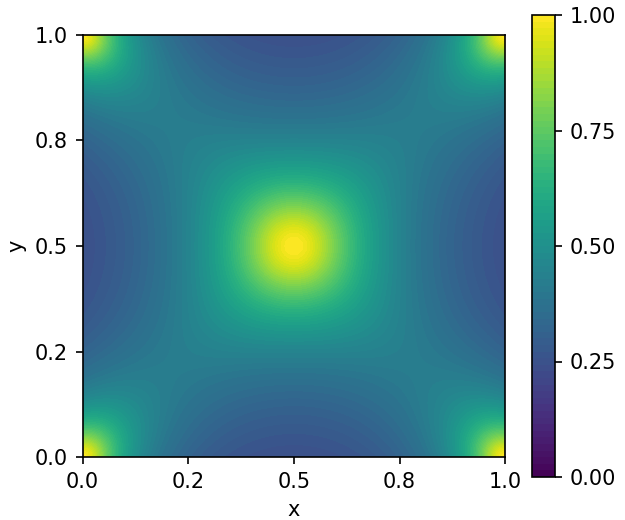
\includegraphics[width=.48\linewidth]{./Images/int_parabole.png}}

    \vspace{0.5em}

    % Légende centrée "Figure X – ..."
    \refstepcounter{figure} % incrémente le compteur de figure
    \centering
    \text{Figure~\thefigure{} – Intensité lumineuse,}
    % Équation centrée juste en dessous
    \[
        I(x, y) = \frac{1}{
            \sqrt{1 + \left(16y(1 - y)(1 - 2x)\right)^2 + \left(16x(1 - x)(1 - 2y)\right)^2}
        }.
    \]
    \label{Fig:int_parabole}
\end{figure}
% insert 2 side by side redimensionned images
\begin{figure}[!htb]
    \begin{minipage}[t]{0.48\textwidth}
        \centering
        \fbox{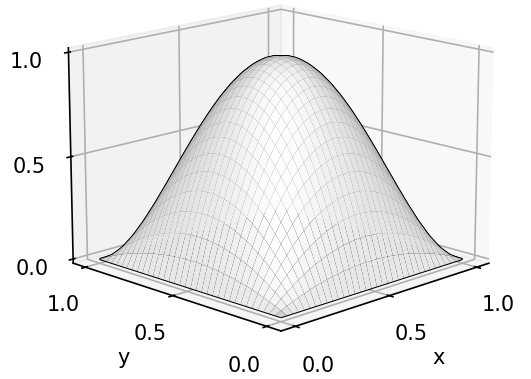
\includegraphics[width=.9\linewidth]{./Images/parabole.png}}
        \caption{Parabole, $101\times101 $ points,\\[0.8ex] \centering$\varepsilon=6.34 \times 10^{-3}$, $n=1730$, $u\left( 
            \dfrac{1}{2},\dfrac{1}{2} \right)=1$.}\label{Fig:parabole}
    \end{minipage}\hfill
    \begin{minipage}[t]{0.48\textwidth}
        \centering
        \fbox{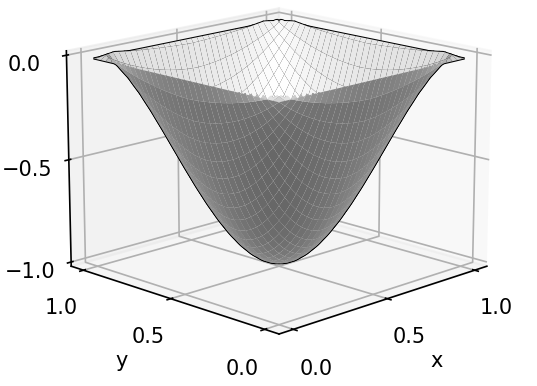
\includegraphics[width=.9\linewidth]{./Images/reverse_parabole.png}}
        \vspace{0.9em}

        % Légende centrée "Figure X – ..."
        \refstepcounter{figure} % incrémente le compteur de figure
        \centering
        \text{Figure~\thefigure{} – Parabole renversée,}\\[0.5em]
        \text{$101 \times 101$ points, $\varepsilon=1.7\times 10^{-2}$, $n=100$,}
        \[
            u\left( \dfrac{1}{2},\dfrac{1}{2}\right) = -1.
        \]\label{Fig:reverse_parabole}
    \end{minipage}
\end{figure}
\newpage
Cet exemple illustre parfaitement le problème d'unicité du problème. En effet, pour une même intensité lumineuse donnée, nous obtenons deux formes différentes en ayant modifié l'information de $u\left(\frac{1}{2},\frac{1}{2} \right)$.

La différence du nombre d'itération nécessaires à la convergence entre les deux figures est flagrante. Nous avons donc cherché une solution pour optimiser le temps de convergence. Nous nous sommes alors rendu compte qu'en modifiant le $U^0$ initial, nous pouvions drastiquement réduire le nombre d'itération. En choisissant $U^0=0$ sur $\p \omb$ et $U^0=1$ dans $\Omega$ nous avons obtenu pour la \textit{Parabole} $n=85$, et $n=100$ pour la \textit{Parabole renversée}. 
Nous pouvons aussi noter une légère différence pour l'erreur, mais nous n'avons pas réussi à déterminer d'où venait cet écart.

\subsubsection{La pyramide}
La \textit{Pyramide} fut le second exemple donné dans le papier. Ici encore, $\omb = \ff{0,1}\times \ff{0,1}$ et nous avons initialisé avec $U^0 = 0$ sur $\omb$. 
\begin{noremark}
    Utiliser le $U^0$ optimal précédent ne change rien à la convergence pour cette figure.
\end{noremark}

% insert 2 side by side redimensionned images
\begin{figure}[!htb]
    \begin{minipage}[t]{0.48\textwidth}
        \centering
        \fbox{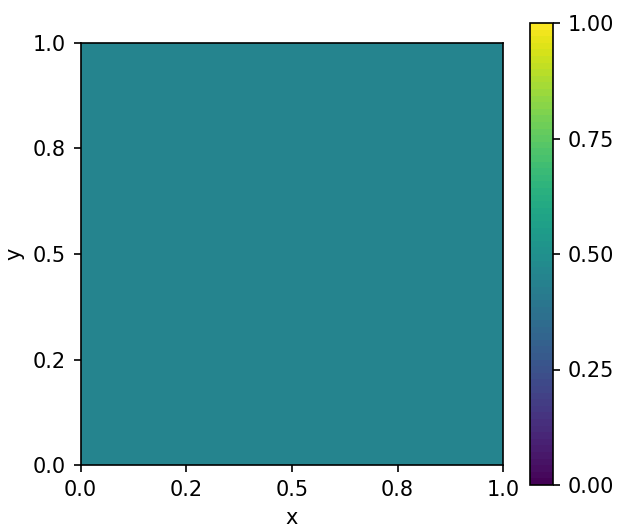
\includegraphics[width=.9\linewidth,height=5.5cm]{./Images/int_pyramide.png}}
        \caption{Intensité lumineuse,  \centering $I(x,y)=\dfrac{1}{\sqrt{5}}.$}\label{Fig:int_pyramide}
    \end{minipage}\hfill
    \begin{minipage}[t]{0.48\textwidth}
        \centering
        \fbox{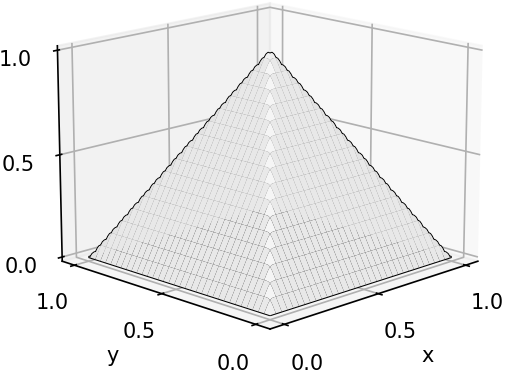
\includegraphics[width=.9\linewidth,height=5.5cm]{./Images/pyramide.png}}
        \caption{Pyramide, $101\times101 $ points, \\[1ex] \centering$\varepsilon=1.65 \times 10^{-4}$, $n=100$.}\label{Fig:pyramide}
    \end{minipage}
\end{figure}
\newpage
Cette figure est particulière. En effet, celle-ci ne possède aucun point d'intensité égale à $1$. D'après ce qui précède, la solution est donc unique. Nous n'avons donc pas besoin de fixer des valeurs à l'intérieur de la grille pour s'assurer de la convergence vers \og la bonne solution \fg.

\subsubsection{Deux autres exemples}
Dans cette dernière sous-section, nous présentons deux exemples illustrant la sensibilité du processus de reconstruction par rapport aux données internes de la grille. Nous avons $\omb = \ff{0,1}\times \ff{0,1}$ et $U^0$ est choisi comme le $U^0$ optimisé des paraboles.

% insert an image as wide as 70% of line length
\begin{figure}[!htb]
    \centering
    \fbox{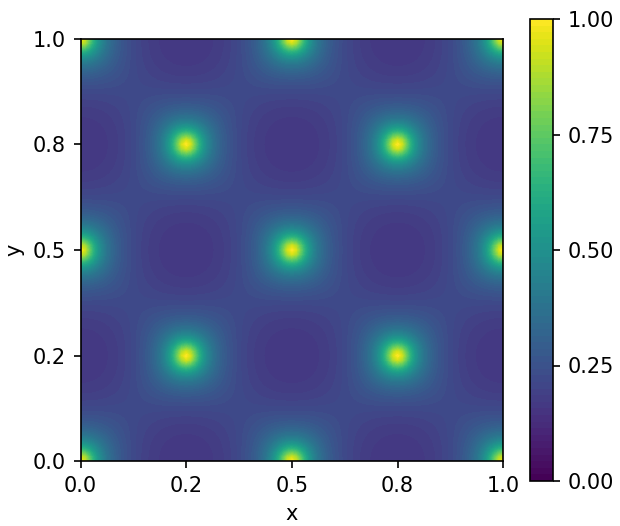
\includegraphics[width=.48\linewidth]{./Images/int_fig78.png}}
    \vspace{0.5em}

    % Légende centrée "Figure X – ..."
    \refstepcounter{figure} % incrémente le compteur de figure
    \centering
    \text{Figure~\thefigure{} – Intensité lumineuse,}
    % Équation centrée juste en dessous
    \[
        I(x, y) = \frac{1}{
            \sqrt{1 + \left(2\pi\sin(2\pi y)\cos(2\pi x)\right)^2 + \left(2\pi\sin(2\pi x)\cos(2\pi y)\right)^2}
        }.
    \]
\end{figure}
\vspace{10cm} % Espacement réduit ici si besoin
% insert 2 side by side redimensionned images
\begin{figure}[!htb]
    \begin{minipage}[t]{0.48\textwidth}
        \centering
        \fbox{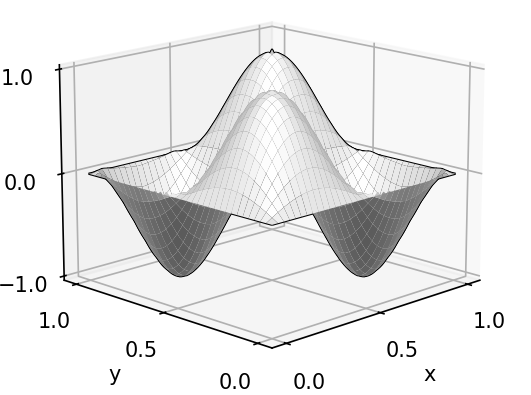
\includegraphics[width=.9\linewidth,height=5.5cm]{./Images/fig7.png}}
        \caption{
            $101\times101 $ points, \\[0.5em] \centering$\varepsilon=6.34\times10^{-3}$, $n = 110$,
            \centering\protect
            $\begin{aligned}
                    u\left(\dfrac{1}{4},\dfrac{3}{4} \right) &= u\left(\dfrac{3}{4},\dfrac{1}{4} \right) = -1, \\
                    u\left(\dfrac{1}{4},\dfrac{1}{4} \right) &= u\left(\dfrac{3}{4},\dfrac{3}{4} \right) = 1, \\
                    u\left(\dfrac{1}{2},\dfrac{1}{2} \right) &= 0.
                \end{aligned}$
        }\label{Fig:fig7}
    \end{minipage}\hfill
    \begin{minipage}[t]{0.48\textwidth}
    \centering\fbox{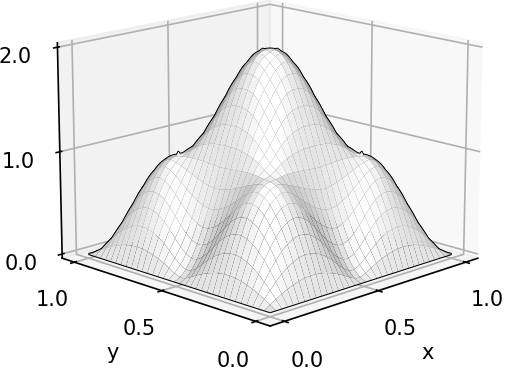
\includegraphics[width=.9\linewidth,height=5.5cm]{./Images/fig8.png}}
        \caption{
            $101\times101 $ points, $n=350,$\\[1ex]
            \centering\protect
            $\begin{aligned}
                u\left(\dfrac{1}{4},\dfrac{3}{4} \right) &= u\left(\dfrac{3}{4},\dfrac{1}{4} \right) = 1, \\
                u\left(\dfrac{1}{4},\dfrac{1}{4} \right) &= u\left(\dfrac{3}{4},\dfrac{3}{4} \right) = 1, \\
                u\left(\dfrac{1}{2},\dfrac{1}{2} \right) &= 2.
            \end{aligned}$
        }\label{Fig:fig8}
    \end{minipage}
\end{figure}


Sur l'intensité lumineuse nous remarquons $5$ points intérieurs d'intensité $1$. Encore une fois, nous devons connaître la hauteur en ces points de la solution pour s'assurer de converger vers la bonne solution étudiée. Nous avons essayé de trouver la solution analytique de la Figure \ref{Fig:fig8} afin de calculer l'erreur. En faisant de grandes intégrations de l'intensité, nous n'avons malheureusement pas trouvé cette solution. C'est pourquoi celle-ci manque à la légende de la  figure. 

\begin{noremark}
    Nous nous sommes rendu compte plus tard que dans le papier de Mme Rouy et Mme Tourin, aucune erreur n'était donnée pour cette figure. Nous en avons déduit qu'elles n'avaient pas réussi non plus à déterminer la solution analytique.
\end{noremark}

\subsection{Résultats supplémentaires}
Dans cette section, nous présentons des résultats complémentaires à ceux donnés dans le papier. En retrouvant au fur et à mesure les figures du papier, nous avons eu l'envie de jouer avec notre code et de tester ses limites. 

Contrairement aux exemples de la section précédente, nous avons ici adopté une approche différente. En effet, l’intensité lumineuse des courbes que nous souhaitions reconstituer n’était pas connue à l’avance. Plutôt que de partir de la lumière renvoyée par l’objet pour en déduire sa forme (comme nous l’avions fait auparavant) nous avons inversé la démarche : à partir de la forme de l’objet, nous avons calculé son gradient afin d’estimer l’intensité lumineuse qu’il renvoie. Cette intensité a ensuite été transmise à notre programme, qui a alors tenté de retrouver la courbure de l’objet initial.

Puisque nous partions des solutions analytiques, nous avons pu calculer l'erreur en norme L1 pour les deux figures que nous allons présenter.


\subsubsection{La demi-parabole}
Jusqu’à présent, nous nous sommes uniquement intéressés à des cas où les formes étudiées possédaient un nombre fini de points critiques. Afin d’évaluer l’influence éventuelle de ce caractère fini sur la qualité de la reconstruction, nous avons cherché à analyser une courbe présentant une infinité de points d’intensité lumineuse égale à 1. L’objectif était de déterminer si le fait que les points critiques soient en nombre dénombrable dans les exemples précédents jouait un rôle dans les performances de notre méthode.

Nous avons alors pensé la fonction $f(x,y) = x^2$ dans $\R^2$. En effet, celle-ci possède un nombre indénombrable de points critiques sur l'axe $x=0$. Nous avons travaillé dans $\omb = \ff{-1,1}\times \ff{-1,1}$ et choisi, $U^0=1$ sur les axes $x=-1$ et $x=1$. Les autres bords sont $U^0=x^2$ sur les axes $y=-1$ et $y=1$. Enfin, dans $\Omega'$, $U^0=0$.

\begin{figure}[!htb]
    \centering
    \begin{minipage}[t]{0.48\textwidth}
        \centering
        \fbox{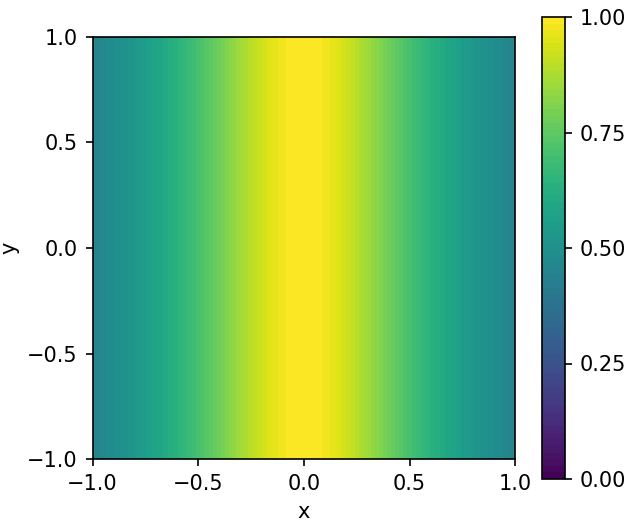
\includegraphics[width=.9\linewidth,height=5.5cm]{./Images/int_x2.png}}
        \caption{Intensité lumineuse,\\[1ex] \centering $I(x,y)=\dfrac{1}{\sqrt{1+{(2x)}^2}}.$}
        \label{Fig:int_x2}
    \end{minipage}%
    \hfill
    \begin{minipage}[t]{0.48\textwidth}
        \centering
        \fbox{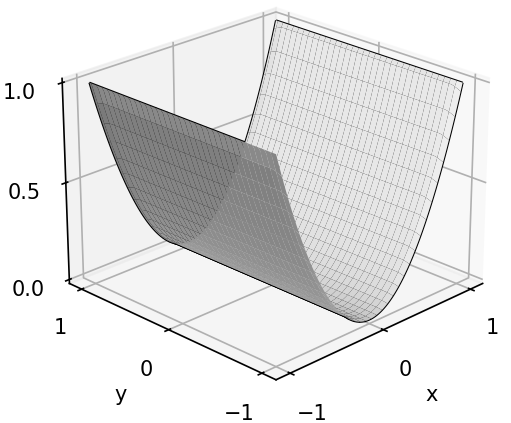
\includegraphics[width=.9\linewidth,height=5.5cm]{./Images/x2.png}}
        \vspace{0.9em}

        % Légende centrée "Figure X – ..."
        \refstepcounter{figure} % incrémente le compteur de figure
        \centering
        \text{Figure~\thefigure{} – $f(x,y)=x^2$,}\\[0.5em]
        \text{$101 \times 101$ points, $\varepsilon=9.75\times 10^{-3}$, $n=80$,}
        \[
            u\big|_{x=0} = 0.
        \]\label{Fig:x2}
    \end{minipage}
\end{figure}

Cet exemple illustre bien le fait que le nombre de points critiques n'est pas un problème pour le schéma numérique. 
Nous avons fait tendre le pas du schéma vers 0 et nous n'avons constaté aucun problème de convergence particulier vers la solution de viscosité. 
\begin{noremark}
    En modifiant les conditions aux bords nous avons aussi réussi à faire converger le programme vers des solutions de viscosités qui avaient perdu leur caractère $C^1$. Nous donnons un exemple de celles-ci en dessous avec $U^0=0$ sur les bords.
\end{noremark}
\vspace{10cm} % Espacement réduit ici si besoin
% insert an image as wide as 70% of line length
\begin{figure}[htb]
    \centering
    \fbox{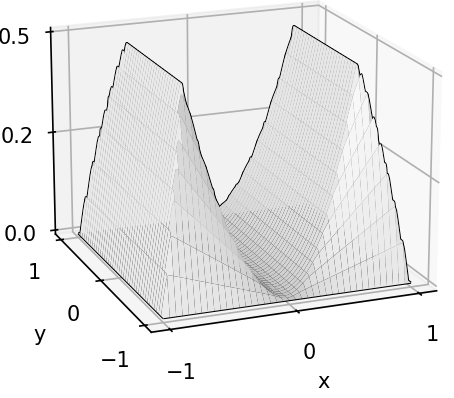
\includegraphics[width=.48\linewidth]{./Images/x2_mixedbd.png}}
    \caption{$101\times 101$ points, $n=275$,  $\left. u\right|_{x=0}=0.$ }\label{Fig:x2_mixedbd}
\end{figure}


\subsubsection{Le vase}
Après avoir étudié un cas présentant une infinité de points critiques, nous avons entrepris la reconstitution d’un \textit{Vase}. Cet objet, plus complexe que les courbes précédemment analysées. Il nous a servis de source de motivation et de compréhension, car c’est en travaillant sur cette forme que nous avons véritablement assimilé les principes du Shape-from-Shading.

Nous avons choisi de présenter cet exemple en dernier, car il s’agit de la forme la plus difficile que nous ayons eu à traiter. Elle constitue à la fois un défi technique et une illustration de l’efficacité de notre méthode. Nous donnons l'intensité lumineuse du \textit{Vase} ainsi que les images de sa reconstruction sous deux angles différents avant de rentrer dans les détails de la complexité.

\begin{figure}[htb]
    \centering
    \fbox{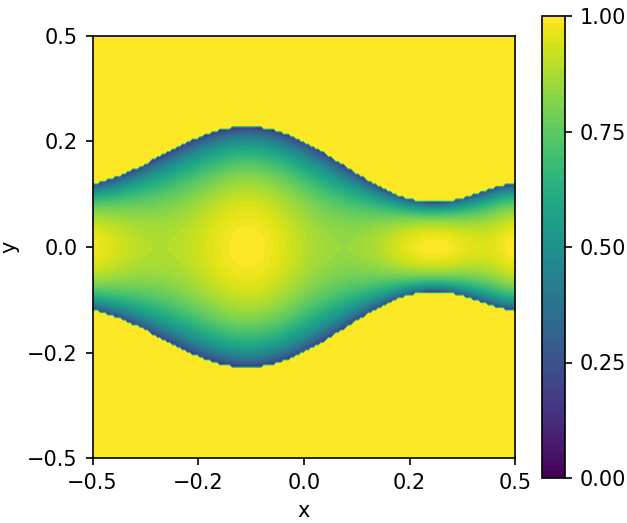
\includegraphics[width=.5\linewidth]{./Images/int_vase.png}}
    \caption{Intensité lumineuse du vase.}\label{Fig:int_vase}
\end{figure}
\vspace{15cm} % Espacement réduit ici si besoin
% insert 2 side by side redimensionned images
\begin{figure}[!htb]
    \begin{minipage}[t]{0.48\textwidth}
        \centering
        \fbox{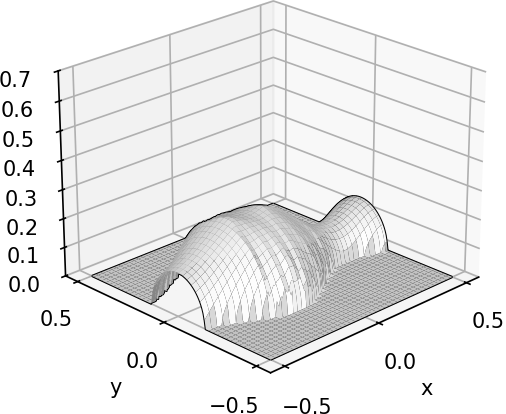
\includegraphics[width=.9\linewidth,height=5.5cm]{./Images/vase_cote.png}}
        \caption{Vase vu de côté.}\label{Fig:vase_cote}
    \end{minipage}\hfill
    \begin{minipage}[t]{0.48\textwidth}
    \centering\fbox{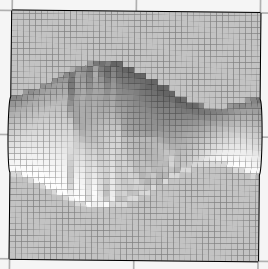
\includegraphics[width=.8\linewidth,height=5.5cm]{./Images/vase_dessus.png}}
        \caption{Vase vu du dessus.}\label{Fig:vase_dessus}
    \end{minipage}
\end{figure}

Pour les deux figures, nous avons travaillé sur $\omb=\ff{-0.5,0.5}\times \ff{-0.5,0.5}$ avec\\ $171\times 171$ points. L'erreur en norme L1 est de $4.12 \times 10^{-3}$ et il a fallu 220 itérations pour converger. 

Nous allons à présent développer les difficultés rencontrées quant à la reconstruction du \textit{Vase}. Nous avons dans un premier temps trouvé l'équation d'un vase en 2D. Sur internet nous avons trouvé l'équation suivante sur $\ff{-0.5,0.5}\times \ff{-0.5,0.5}$
\begin{align}
    vase(x,y) =\left\{
    \begin{array}{ll}
         \mathopen{}\sqrt{P(x)^2 -y^2} & \ \text{si } P(x)^2-y^2>0\\  
         0& \ \text{sinon }
    \end{array}
    \right.
\end{align}
où $P(x) = 0.15 - 0.025(6x- 1) (2x - 1)^2 (3x + 2)^2 (2x + 1)$.

Nous avons ensuite calculé les dérivées partielles de cette fonction et en avons déduit l'intensité lumineuse de notre objet. Nous ne donnerons pas l'expression explicite de celle-ci. Nous avons alors longtemps bloqué sur la reconstruction, en effet, le \textit{Vase} ne recouvre pas le carré en entier. Ainsi, il a fallu donner des conditions aux bords différentes de celles qu'on utilisait précédemment. Nous avons donc dû donner au programme les valeurs exactes du \textit{Vase} sur les axes $x=-0.5$ et $x=0.5$ ainsi que sur les points intérieurs d'intensité 1. Il n'a pas été facile de lier toutes les conditions entre elles. 

Comme nous pouvons le constater sur la Figure \ref{Fig:int_vase}, il y a beaucoup de points ayant une intensité lumineuse proche de 1. Cela joue une importance particulière sur la reconstruction de la partie centrale du \textit{Vase} qui présente certaines imperfections (voir Figure \ref{Fig:vase_cote} et Figure \ref{Fig:vase_dessus}). En effet, puisque celui-ci est assez plat, de nombreuses erreurs d'arrondi ont lieu dans cette zone. Nous avons rencontré quelques difficultés liées à ces erreurs d'arrondi que nous avons donc dû gérer du mieux possible. Actuellement, notre programme met toujours beaucoup de temps à converger dans cette partie du \textit{Vase}.

\begin{noremark}
    Nous pouvons voir sur la Figure \ref{Fig:int_vase} que toute la partie en dehors du \textit{Vase} possède une intensité lumineuse égale à 1. C'est un choix de notre part. Il était plus facile pour nous de considérer cette zone externe comme une partie du \textit{Vase}, mais avec une hauteur de 0. En effet, nous aurions pu fixer l'intensité lumineuse du \textit{Vase} dans cette partie comme  \og NAN \fg{} (Not A Number) ce qui donnerait quelque chose de plus cohérent. Mais cela aurait engendré de gros changements dans notre code pour le même résultat. 
\end{noremark}



\subsection{Comparaison des algorithmes}
Tous les résultats présentés dans la section précédente ont été obtenus à l’aide du schéma explicite basé sur l’algorithme du point fixe. Nous souhaitons à présent mettre en évidence l’efficacité de l’algorithme \eqref{algo_papier} proposé dans l’article. Pour cela, nous allons comparer les deux méthodes en termes de nombre d’itérations nécessaires à la convergence, ainsi que de l’erreur relative entre les solutions obtenues avec \eqref{pt_fixe} et avec \eqref{algo_papier}. Nous n'allons pas revoir tous les exemples précédents. Nous avons sélectionné les exemples les plus pertinents illustrant la performance de l'algorithme du papier et mis les informations importantes dans un tableau que nous commenterons. 

Les trois exemples ci-dessous ont été retrouvés avec les mêmes conditions initiales qu'avant. Les intensités lumineuses sont aussi identiques à celles utilisées plus tôt dans notre rapport.
\begin{figure}[!htb]
    \centering
    \begin{minipage}[t]{0.48\textwidth}
        \centering
        \fbox{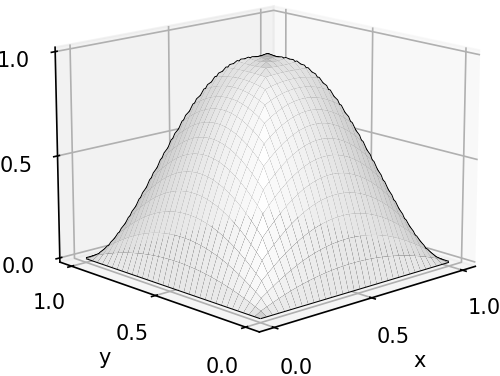
\includegraphics[width=.9\linewidth,height=5.5cm]{./Images/parabole_opti.png}}
        \caption{Parabole obtenue avec \\ \centering l'algorithme du papier, $101\times101$ points.}
        \label{Fig:parabole_opti}
    \end{minipage}%
    \hfill
    \begin{minipage}[t]{0.48\textwidth}
        \centering
        \fbox{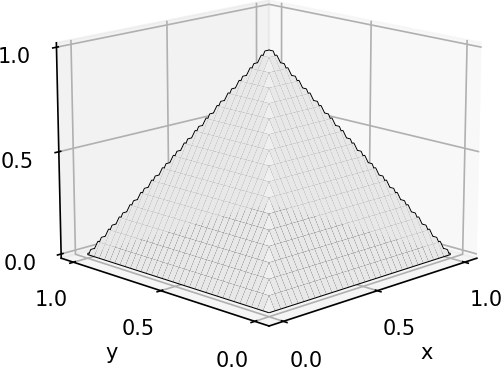
\includegraphics[width=.9\linewidth,height=5.5cm]{./Images/pyramide_opti.png}}
        \caption{Pyramide obtenue avec \\ \centering l'algorithme du papier, $101\times101$ points.}
        \label{Fig:pyramide_opti}
    \end{minipage}
\end{figure}
\begin{figure}[!ht]
\centering
    \begin{minipage}[t]{0.48\textwidth}
        \centering
        \fbox{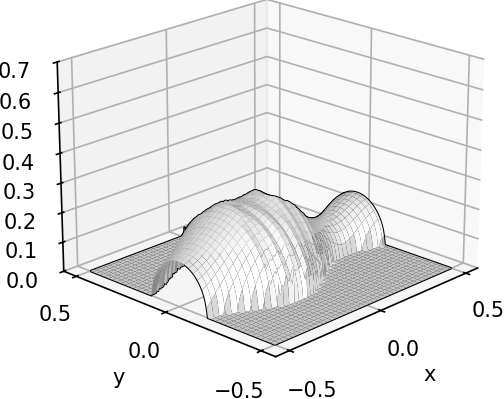
\includegraphics[width=.95\linewidth,height=5.5cm]{./Images/vase_opti.png}}
        \caption{Vase obtenu avec \\ \centering l'algorithme du papier, $171\times171$ points.}
        \label{Fig:vase_opti}
    \end{minipage}
\end{figure}

\begin{figure}[!htb] 
    \centering
    \renewcommand{\arraystretch}{1.5} % pour espacer verticalement
    \begin{tabular}{|c|c|c|c|c|}\hline
         & $\varepsilon$ point fixe & $\varepsilon$ algorithme & $n$ point fixe & $n$ algorithme \\ \hline
        Parabole & $6.34 \times 10^{-3}$ & $7.52 \times 10^{-3}$ & 85 & 48 \\ \hline
        Pyramide & $1.65 \times 10^{-4}$ & $1.16 \times 10^{-16}$ & 100 & 49\\ \hline
        Vase     & $4.12 \times 10^{-3}$ & $2.85 \times 10^{-3}$ & 220 & 90 \\  \hline
    \end{tabular}
    \caption{Comparaison du nombre d'itérations et de l'erreur pour les deux méthodes.}
    \label{fig:comparaison_algo}
\end{figure}

La première différence notable que l'on observe sur la figure \ref{Fig:parabole_opti} est l'apparence plus linéaire de la \textit{Parabole}. En effet, ses bords ainsi que son sommet sont bien moins arrondis que ceux de la \textit{Parabole} reconstruite avec \eqref{pt_fixe} (voir Figure \ref{Fig:parabole}). On peut d'ailleurs voir que cela se ressent en regardant l'erreur des deux paraboles. En effet, bien que l'algorithme \eqref{algo_papier} converge 1,7 fois plus vite, l'erreur en norme L1 de notre \textit{Parabole} est légèrement plus élevée ici que la première (Elles sont presque égales).

Pour la \textit{Pyramide}, nous observons à nouveau une différence graphique. Cependant, celle-ci est bien plus subtile que pour la \textit{Parabole}. En effet, à la place d'avoir des pentes presque lisses, celle-ci présente de légères \og marches d'escaliers \fg{} (voir Figure \ref{Fig:pyramide_opti}). En opposition à la \textit{Parabole}, la différence entre les deux erreurs est flagrante. En effet, l'erreur est $10^{12}$ fois plus petite pour l'algorithme du papier. Le nombre d'itérations nécessaires à la convergence est de seulement de $49$, soit deux fois moins que pour l'algorithme du point fixe. On comprend donc que pour la \textit{Pyramide}, l'algorithme \eqref{algo_papier} est en tout point plus performant.

Lorsque l'on reconstruit le \textit{Vase} avec notre algorithme, on observe que la convergence nécessite $2.4$ fois moins d'itérations qu'avec l'algorithme \eqref{pt_fixe}. Cependant, cela se produit au prix d'un résultat graphique moins esthétique. En effet, observe une certaine imperfection au niveau de la zone la plus haute du \textit{Vase}. Cela est encore du aux erreurs d'arrondis dans cette zone presque plate.

L'algorithme du papier est donc bien plus performant d'un point de vue itératif que l'algorithme du point fixe. Quand à l'erreur, elle est inférieure ou équivalente à celle du point fixe. On retiendra tout de même la capacité de \eqref{pt_fixe} à obtenir des résultats plus lisses et plus proches (visuellement parlant) du véritable objet.\\

Nous allons à présent illustrer un exemple sur lequel l'algorithme \eqref{algo_papier} ne fonctionne pas totalement. Il s'agit de la Figure $\ref{Fig:fig7}$. 
\begin{figure}[!ht]
\centering
    \begin{minipage}[t]{0.48\textwidth}
        \centering
        \fbox{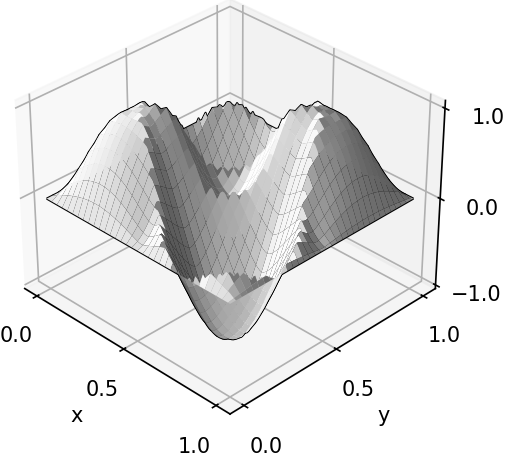
\includegraphics[width=.9\linewidth,height=5.5cm]{./Images/fig7_opti.png}}
        \caption{Mauvaise convergence obtenue avec l'algorithme du papier, \\[1ex] \centering  $101\times101$ points}
        \label{Fig:fig7_opti}
    \end{minipage}
\end{figure}
\newpage
Pour cette reconstruction, l'erreur est $9.83 \times 10^{-2}$ et l'algorithme a convergé en $50$ itérations. L'erreur est donc bien plus grande que celle obtenue avec la reconstruction par la méthode du point fixe (l'erreur était de $6.34 \times 10^{-3}$). Graphiquement parlant, on voit facilement d'où vient ce problème. En effet, les pentes des sommets ne sont pas bombées mais bien creuse. L'algorithme \eqref{algo_papier} semble ne pas réussir à approcher correctement cette partie de la Figure \ref{Fig:fig7_opti}.

\begin{noremark}
    Nous n'avons pas réussi à déterminer clairement pourquoi est-ce que l'algorithme \eqref{algo_papier} n'arrivait pas à converger dans ce cas-là. Il se pourrait que nous atteignions les limites de l'algorithme \eqref{algo_papier}. En effet, peut-être que la formule \og inventée \fg{} par ChatGPT n'est valable que dans certaines situations/hypothèses. \\ 
    Il se pourrait aussi que nous ayons une erreur dans notre code, mais cela serait assez surprenant car celui-ci fonctionne pour le reste des figures.
\end{noremark}




 % Les différents résultats numériques que l'on a obtenu et comparaison entre les algorithmes 
\newpage

\section{Conclusion}

Dans ce rapport, nous avons étudié le problème du Shape-from-Shading à travers l’approche proposée par Rouy et Tourin dans \cite{Rouy_et_Turin}. En nous appuyant sur la théorie des solutions de viscosité pour les équations d’Hamilton-Jacobi, nous avons pu à la fois justifier l'existence et l'unicité d'une solution dans un cadre théorique bien défini et construire un schéma numérique convergent permettant une reconstruction efficace des surfaces.\\

L’étude théorique menée sur l’Hamiltonien nous a permis de trouver une contrainte sur l’intensité lumineuse pour garantir l’unicité afin d'assurer une bonne formulation du problème. Nous avons ensuite étudié deux algorithmes numériques, dont un schéma du point fixe explicite, pour approcher la solution. 

Les résultats numériques obtenus, aussi bien sur les exemples du papier que sur nos propres tests, confirment la robustesse de l’approche. En particulier, nous avons observé le problème d’unicité lorsque l’intensité lumineuse atteint sa valeur maximale. Nous avons aussi pu étudier les limites de nos algorithmes. En effet, l'algorithme du point fixe présentait une efficacité indéniable, mais sa convergence était plutôt lente. L'algorithme donné dans le papier est au contraire plus rapide, mais apporte des résultats moins esthétiques. \\

Ce projet a donc été l’occasion d’explorer un problème à la croisée des mathématiques appliquées, de la vision par ordinateur et de l’analyse numérique. L’étude initiale de ce papier nous a permis de consolider nos compétences de travail en autonomie face à une problématique à la fois nouvelle et complexe. 

Une progression naturelle de ce travail consisterait à étudier des variantes plus réalistes du problème initial, comme l’étude d'objets éclairés par plusieurs sources de lumière, de scènes plus complexes avec plusieurs objets à reconstruire, ou encore l'intégration de modèles non lambertiens.


   % Conclusion et persperctives futures
\newpage

\begin{thebibliography}{MMM99}
\bibitem[1]{Barles_et_Souganidis}
    G. Barles, P.E. Souganidis, \textit{Convergence of approximation schemes for fully nonlinear second
order equations}, 1991, Asymptotic Anal.4, pp. 271-283.
\bibitem[2]{Barles}
    G. Barles, \textit{Solution de viscosité des équations de Hamilton-Jacobi}, 1994, Springer Berlin, Heidelberg. 
\bibitem[3]{lion}
    M.G. Crandall, P.L. Lions, (1983), \textit{Viscosity solutions of Hamilton-Jacobi equations}, May 1983, transactions of the american mathematical society, Volume 277, Number 1.
\bibitem[4]{ref_vase}
    J.D. Durou, M. Falcone, M. Sagona, \textit{Numerical Methods for Shape-from-shading: A New Survey with Benchmarks}, Computer Vision and Image Understanding, 2008, 109 (1), pp.22–43, hal-04587417.
\bibitem[5]{Horn 1975}
    B.K.P. Horn, \textit{The Psychology of Computer Vision}, 1975, Pergamon Press, Vol 8, pp. 19.
\bibitem[6]{Horn 1986}
    B.K.P. Horn, \textit{Robot Vision}, 1986, MIT Eng. Comput. Sci. Ser., MIT Press, McGraw-Hill, New York.
\bibitem[7]{Lions}
    P.L. Lions, \textit{Generalized Solutions of Hamilton-Jacobi Equations}, 1982, Pitman, London.
\bibitem[8]{Osher_et_Rudin}
    S.J. Osher, L. Rudin, \textit{Rapid convergence of approximate solutions to shape-from-shading problem}, à paraître.
\bibitem[9]{Rouy_et_Turin}
    E. Rouy, A. Tourin, \textit{A viscosity solutions approach to Shape-from-Shading}, June 1992, SIAM J. NUMER. ANAL. Vol. 29, No. 3, pp. 867-884.
\end{thebibliography} % la bibliographie
\newpage 


\end{document}

